\RequirePackage[thinlines]{easybmat} %-- muss aufgrund eines Bugs vor etex und tikz geladen werden
\documentclass[a4paper, twoside, headsepline, index=totoc,toc=listof, fontsize=10pt, cleardoublepage=empty, headinclude, DIV=13, BCOR=13mm, titlepage]{scrartcl}
\usepackage{scrtime} % KOMA, Uhrzeit ermoeglicht
\usepackage{scrpage2} % wie fancyhdr, nur optimiert auf KOMA-Skript, leicht andere Syntax
\usepackage{etoolbox}
\usepackage{ifxetex}

%--Farbdefinitionen
%-- muss vor tikz geladen werden
\usepackage[usenames, table, x11names]{xcolor}
\definecolor{dark_gray}{gray}{0.45}
\definecolor{light_gray}{gray}{0.6}

%--Zum Zeichnen
%-- muss vor polyglossia bzw. babel geladen werden
\usepackage{tikz}
\usepackage{tikz-cd}
\usetikzlibrary{external}
\tikzset{>=latex}
\usetikzlibrary{shapes,arrows,intersections}
\usetikzlibrary{calc,3d}
\usetikzlibrary{decorations.pathreplacing,decorations.markings}
\usetikzlibrary{angles}

%-- Konfiguration von tikzexternalize
\tikzexternalize[prefix=tikz/, up to date check=diff]

\ifxetex
\tikzset{external/system call={xelatex \tikzexternalcheckshellescape %-- verwende LuaLaTeX, wegen dynamischer Speicherallokation
    -halt-on-error -interaction=batchmode -jobname "\image" "\texsource"}}
\else
\tikzset{external/system call={pdflatex \tikzexternalcheckshellescape 
    -halt-on-error -interaction=batchmode -jobname "\image" "\texsource"}}
\fi

%-- tikzexternalize fuer tikzcd deaktivieren, da inkompatibel
\AtBeginEnvironment{tikzcd}{\tikzexternaldisable}
\AtEndEnvironment{tikzcd}{\tikzexternalenable}

%-- um Inkompatibilitaeten von quotes und polyglossia bzw. babel zu vermeiden
\tikzset{
  every picture/.append style={
    execute at begin picture={\shorthandoff{"}},
    execute at end picture={\shorthandon{"}}
  }
}
\usetikzlibrary{quotes}
\usepackage{pgfplots}
\pgfplotsset{compat=1.10}



%-- Mathe
\usepackage{mathtools} % beinhaltet amsmath
\mathtoolsset{showonlyrefs, centercolon}
\usepackage{wasysym}
\usepackage{amssymb} %zusätzliche Symbole
\usepackage{latexsym} %zusätzliche Symbole
\usepackage{stmaryrd} %für Blitz
\usepackage{nicefrac} %schräge Brüche
\usepackage{cancel} %Befehle zum Durchstreichen
\usepackage{mathdots}
\DeclareSymbolFont{bbold}{U}{bbold}{m}{n}
\DeclareSymbolFontAlphabet{\mathbbold}{bbold}
\newcommand{\mathds}[1]{\mathbb{#1}} %Um Kompatibilitaet mit frueheren Benutzung von dsfont herzustellen
\newcommand{\ind}{\mathbbold{1}} % charakteristische-Funktion-Eins
\def\mathul#1#2{\color{#1}\underline{{\color{black}#2}}\color{black}} %farbiges Untersteichen im Mathe-Modus

%-- Alles was mit Schrift und XeteX zu tun hat
\ifxetex
    % XeLaTeX
	\usepackage{mathspec} %beinhaltet fontspec 
    \usepackage{polyglossia} %babel-ersatz
    \setmainlanguage[spelling=new,babelshorthands=false]{german}
	\newcommand\glqq{"}
	\newcommand\grqq{"}
	\defaultfontfeatures{Mapping=tex-text, WordSpace={1.4}} %
    \setmainfont[Ligatures=Common, BoldFont={* Bold}, ItalicFont={* Light Italic}]{Source Sans Pro}
	\setsansfont[Scale=MatchLowercase,Ligatures=Common, BoldFont={* Medium}]{Ubuntu}
	\setallmonofonts[Scale=MatchLowercase, ItalicFont={*}]{Consolas} 
	\usepackage{xltxtra}
	\usepackage{fontawesome}
\else
    % default: pdfLaTeX
    \usepackage[ngerman]{babel}
    \usepackage[T1]{fontenc}
    \usepackage[utf8]{inputenc}
	\usepackage{textcomp} %verhindert ein paar Fehler bei den Fonts
    \usepackage[babel=true, tracking=true]{microtype}
	\usepackage{lmodern}
	\renewcommand{\familydefault}{\sfdefault} 
\fi


%--Mixed
\usepackage[neverdecrease]{paralist}
\usepackage[german=quotes]{csquotes}
\usepackage{makeidx}
\usepackage{booktabs}
\usepackage{wrapfig}
\usepackage{float}
\usepackage[margin=10pt, font=small, labelfont=sf, format=plain, indention=1em]{caption}
\captionsetup[wrapfigure]{name=Abb. }
\usepackage{stackrel}
\usepackage{ifthen}
\usepackage{multicol}
\flushbottom

%--Hyphenation
\hyphenation{di-men-si-o-na-le}


%--Unterstreichung
\usepackage[normalem]{ulem}
\setlength{\ULdepth}{1.8pt}

%--Indexverarbeitung
\newcommand{\bet}[1]{\textbf{#1}}
\newcommand{\Index}[1]{\textbf{#1}\index{#1}}
\makeindex
\setindexpreamble{{\noindent \itshape Die \emph{Seitenzahlen} sind mit Hyperlinks zu den entsprechenden Seiten versehen, also anklickbar} \ifxetex \faHandUp\fi \par \bigskip}
\renewcommand{\indexpagestyle}{scrheadings}


%--Marginnote & todonotes
\usepackage{marginnote}
\renewcommand*{\marginfont}{\color{dark_gray} \itshape \footnotesize }
\usepackage[textsize=small]{todonotes}
\makeatletter
\renewcommand{\todo}[2][]{\tikzexternaldisable\@todo[#1]{#2}\tikzexternalenable}
\makeatother

%--Konfiguration von Hyperref pdfstartview=FitH, 
\usepackage[hidelinks, pdfpagelabels,  bookmarksopen=true, bookmarksnumbered=true, linkcolor=black, urlcolor=SkyBlue2, plainpages=false, hypertexnames=false, citecolor=black, hypertexnames=true, pdfauthor={Jannes Bantje}, pdfborderstyle={/S/U}, linkbordercolor=SkyBlue2, colorlinks=false]{hyperref}

\let\orighref\href
\ifxetex
\renewcommand{\href}[2]{\orighref{#1}{#2\,\faExternalLink}}
\renewcommand{\url}[1]{\href{#1}{\nolinkurl{#1}}}
\fi


%--Römische Zahlen
\newcommand{\RM}[1]{\MakeUppercase{\romannumeral #1{}}}

%--Punkte (nach hyperref)
\usepackage{ellipsis}

%%--Abkürzungen etc.
\newcommand{\light}{\text{\Large $\lightning$}}

%-- Definitionen von weiteren Mathe-Befehlen
\DeclareMathOperator{\re}{Re} %Realteil
\DeclareMathOperator{\im}{Im} %Imaginaerteil
\DeclareMathOperator{\id}{id} %identische Abbildung
\DeclareMathOperator{\Sp}{Sp} %Spur
\DeclareMathOperator{\sgn}{sgn} %Signum
\DeclareMathOperator{\alt}{Alt} %Alternierende n-linearFormen
\DeclareMathOperator{\End}{End} %Endomorphismen
\DeclareMathOperator{\Vol}{Vol} %Volumen
\DeclareMathOperator{\dom}{dom} %Domain
\DeclareMathOperator{\Hom}{Hom} %Homomorphismen
\DeclareMathOperator{\bild}{Bild} %Bild
\DeclareMathOperator{\Kern}{Kern }
\DeclareMathOperator{\rg}{rg} %Rang
\DeclareMathOperator{\Rg}{Rg} %Rang
\DeclareMathOperator{\diam}{diam} %Durchmesser
\DeclareMathOperator{\dist}{dist} %Distanz
\DeclareMathOperator{\grad}{grad} %Gradient
\DeclareMathOperator{\dive}{div} %Gradient
\DeclareMathOperator{\rot}{rot} %Rotation
\DeclareMathOperator{\hess}{Hess} %Hesse-Matrix
\DeclareMathOperator{\koker}{Koker} %Kokern
\DeclareMathOperator{\aut}{Aut} %Automorphismen
\DeclareMathOperator{\ord}{ord} %Ordnung
\DeclareMathOperator{\ggT}{ggT} %ggT
\DeclareMathOperator{\kgV}{kgV} %kgV
\DeclareMathOperator{\Gr}{Gr} %Gerade
\DeclareMathOperator{\Kr}{Kr} %Kreis
\DeclareMathOperator{\Char}{char} %Charakteristik
\DeclareMathOperator{\Aut}{Aut} %Automorphismen
\DeclareMathOperator{\D}{D} %formale Ableitung
% \DeclareMathOperator{\mathd}{d} %formale Ableitung
\newcommand{\mathd}{\ensuremath{\mathrm{d}}}
\DeclareMathOperator{\cov}{cov} %Kovarianz
\DeclareMathOperator{\Gal}{Gal} %Galois
\DeclareMathOperator{\supp}{supp} %Träger
\DeclareMathOperator{\Sym}{Sym} %Symmetrische Gruppe
\DeclareMathOperator{\Zyl}{Zyl} %Zylinder
\DeclareMathOperator{\Mod}{Mod} %Moduln
\DeclareMathOperator{\EPK}{EPK} %Einpunktkompaktifizierung
\DeclareMathOperator{\conj}{conj} %Konjugation
\DeclareMathOperator{\ann}{ann} %Annulator
\DeclareMathOperator{\tor}{tor} %Torsionsmodul
\DeclareMathOperator{\Int}{Int} %Interior/Inneres
\DeclareMathOperator{\Br}{Br} %Brauerergruppe
\DeclareMathOperator{\GL}{GL} %allgemeine lineare Gruppe
\DeclareMathOperator{\Tr}{Tr} %Spur/Trace
%\DeclareMathOperator{\op}{op} %entgegengesetzter Ring
\newcommand{\op}{\mathrm{op}}

\newcommand{\Ker}{\ensuremath{\Kern \,}}
\newcommand{\zirkel}{\rotatebox[origin = c]{-90}{$\varangle$}}
\newcommand{\wirkung}{\!\curvearrowright\!}

\newcommand{\oE}{\OE}

%--Beweisende
\newcommand{\bewende}{\ifmmode \tag*{$\square$} \else \hfill $\square$ \fi}

%--Volumen
\newcommand{\vol}[1]{\ensuremath{\Vol_{#1}}}

%--Skalarprodukt
\DeclarePairedDelimiterX\sprod[2]{\langle}{\rangle}{#1\,\delimsize\vert\,#2}

%--Betrag, Gaußklammer
\DeclarePairedDelimiter{\abs}{\lvert}{\rvert}
\DeclarePairedDelimiter{\ceil}{\lceil}{\rceil}

%--Norm
\DeclarePairedDelimiter\doppelstrich{\Vert}{\Vert}
\newcommand{\norm}[2][\relax]{
\ifx#1\relax \ensuremath{\doppelstrich*{#2}}
\else \ensuremath{\doppelstrich*{#2}_{#1}}
\fi}


%--Umklammern
\DeclarePairedDelimiter\enbrace{(}{)}
\DeclarePairedDelimiter\benbrace{[}{]}

%--Mengen
\DeclarePairedDelimiterX\mengenA[1]{\lbrace}{\rbrace}{#1}
\DeclarePairedDelimiterX\mengenB[2]{\lbrace}{\rbrace}{#1\, \delimsize\vert \, #2}

\makeatletter
\newcommand{\set}[2][\relax]{
\ifx#1\relax \ensuremath{
\mengenA*{#2}}
\else \ensuremath{%
  \mengenB*{#1}{#2}}
\fi}
\makeatother


%--offen und abgeschlossen
\newcommand{\off}{\! \stackrel[\text{offen}]{}{\subset} \!}
\newcommand{\abg}{\! \stackrel[\text{abg.}]{}{\subset} \!}

%--Differential
\newcommand{\diff}[2]{\ensuremath{\frac{{\partial #1}}{{\partial #2}} }}
\newcommand{\diffd}[2]{\ensuremath{\frac{\mathrm{d} #1}{\mathrm{d} #2} }}

%--Diagonale Linien für Matrizen
\newcommand\tikzmark[1]{%
  \tikz[overlay,remember picture,baseline] \node [anchor=base] (#1) {};}

\newcommand\MyLine[3][]{%
  \begin{tikzpicture}[overlay,remember picture]
    \draw[#1] (#2.south) -- (#3.north);
  \end{tikzpicture}}
  
%--Jordankasten
\newcommand{\Jord}{ \begin{BMAT}{|ccc|}{|ccc|} %
				0 & & \\ %
				1\tikzmark{z} &  \diagdown & \\ %
				& \tikzmark{u}1 \MyLine[thick]{z}{u} &  0 %
			\end{BMAT}}
			
%--Jordankasten mit Lambda
\newcommand{\JordLa}[1][\empty]{%
	\ifthenelse{\equal{#1}{\empty}}
		{\begin{BMAT}{|ccc|}{|ccc|} %
				\lambda & & \\ %
				1\tikzmark{z} &  \diagdown & \\ %
				& \tikzmark{u}1 \MyLine[thick]{z}{u} &  \lambda  %
			\end{BMAT}}
		{\begin{BMAT}{|ccc|}{|ccc|} %
				\lambda_{#1}  & & \\ %
				1\tikzmark{z} &  \diagdown & \\ %
				& \tikzmark{u}1 \MyLine[thick]{z}{u} &  \lambda_{#1}  %
			\end{BMAT}}}

%--Inhaltsverzeichnis
\usepackage[tocindentauto]{tocstyle}
\usetocstyle{KOMAlike}			

\newcommand{\fach}{Höhere Algebra \RM{1}}
%\newcommand{\shortFach}{Analysis, Topologie, Geometrie}

\newcommand{\prof}{Prof.\,Dr.\,Dr.\,Katrin Tent}


%--Konfiguration von scrheadings
\setheadsepline{1pt}[\color{light_gray}]
\pagestyle{scrheadings}
%\fancyhf[H, F]{}
\clearscrheadfoot

\providecommand{\shortFach}{\fach}
\lehead{ 
\includegraphics[height=0.5 cm,keepaspectratio]{../master/Bilder/Logo_WWU_Muenster_light_gray.pdf}}
\rehead{\rule{0cm}{0.5cm}\footnotesize \sffamily \color{light_gray} Jannes Bantje -- Mitschrift \shortFach}
\lohead{\rule{0cm}{0.5cm} \footnotesize \sffamily \color{light_gray} Stand: \today \; \thistime[:]}
\rohead{
\includegraphics[height=0.5 cm,keepaspectratio]{../master/Bilder/fb10logo_gray.pdf}}


\ofoot[{ \color{dark_gray} \LARGE \sffamily \thepage}]{{ \color{dark_gray} \LARGE \sffamily \thepage}} %hier wir auch der plain Stil bearbeitet!
\automark{section}
\ifoot{ \color{dark_gray} \small \leftmark}

%--Metadaten
\author{Jannes Bantje}
\titlehead{
\includegraphics[height=1.5cm, keepaspectratio]{../master/Bilder/Logo_WWU_Muenster.pdf}%
\hfill 
\includegraphics[height=1.3cm, keepaspectratio]{../master/Bilder/fb10logo.pdf}}
\title{Skript \fach}
\subtitle{Mitschrift der Vorlesung  \enquote{\fach} von \prof}

\publishers{
Aktuelle Version verfügbar bei: \bigskip\\
\normalsize
\begin{minipage}[t]{0.45\textwidth}
	\centering{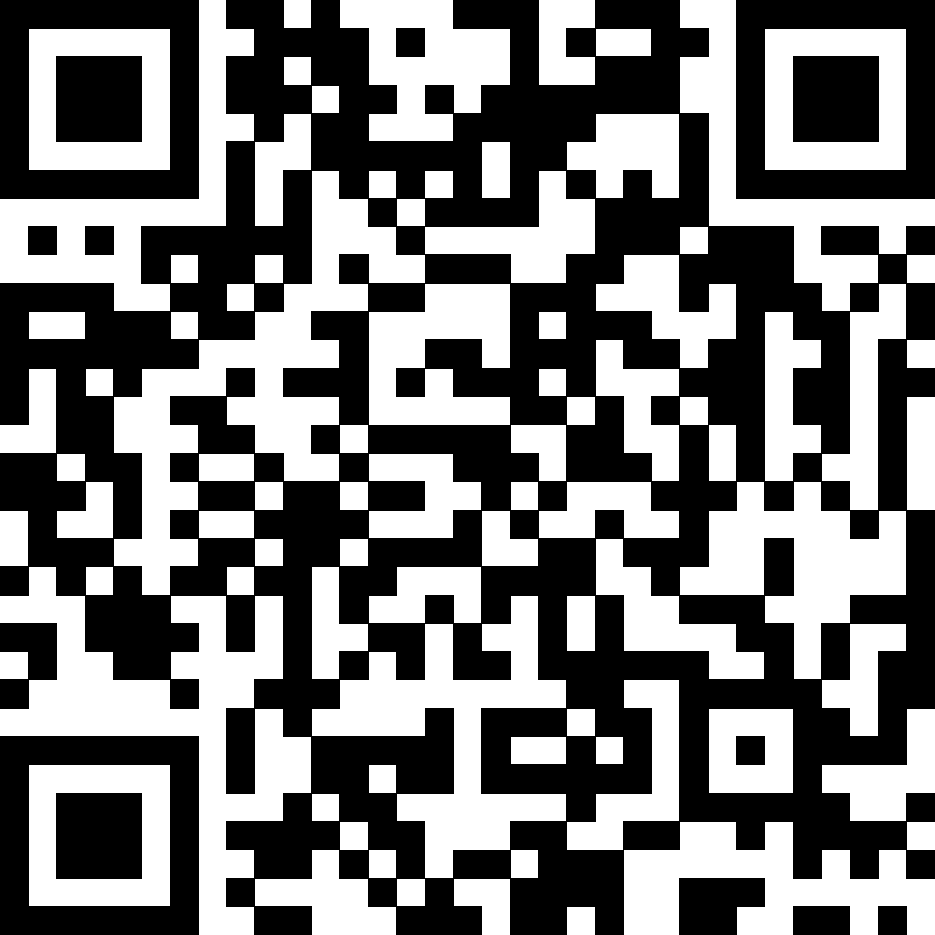
\includegraphics[width=3cm, keepaspectratio]{../master/Bilder/qr_github.pdf} \medskip\\
	
\includegraphics[height=0.4cm, keepaspectratio]{../master/Bilder/github_octo.pdf} 
	
\includegraphics[height=0.4cm, keepaspectratio]{../master/Bilder/GitHub_Logo.pdf} (inklusive Sourcecode)\\
	{\small\url{https://github.com/JaMeZ-B/latex-wwu}}}
\end{minipage}
\hfill
\begin{minipage}[t]{0.45\textwidth}
	\centering{
	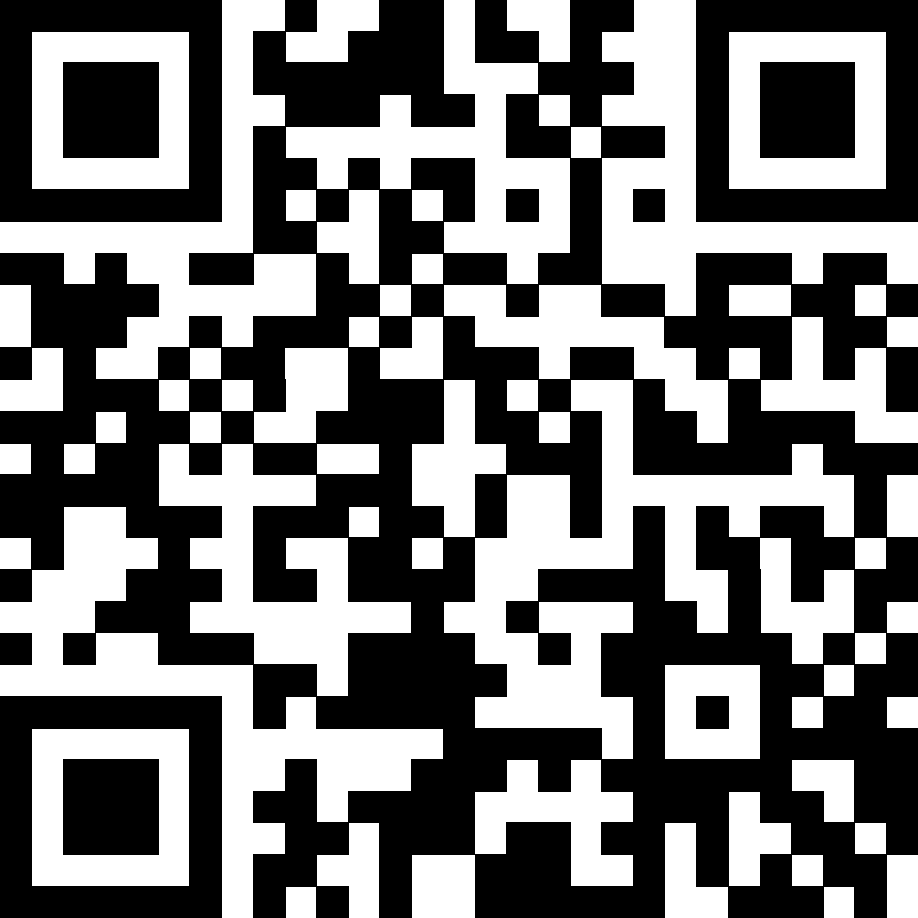
\includegraphics[width=3cm, keepaspectratio]{../master/Bilder/qr_btsync.pdf} \medskip\\
	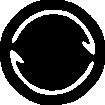
\includegraphics[height=0.4cm, keepaspectratio]{../master/Bilder/bt_sync_logo.pdf} 
	{\large \textbf{Bittorrent} Sync} \\
	\texttt{B6WH2DISQ5QVYIRYIEZSF4ZR2IDVKPN3I}
	}
\end{minipage}
}


\begin{document}
\maketitle
\pagenumbering{Roman}

\tableofcontents
\cleardoubleoddemptypage

\pagenumbering{arabic}
\setcounter{page}{1}


\bet{Literatur:}
\begin{itemize}
	\item P.M. Cohn: Basic Algebra, (Further Algebra) Springer
	\item N. Jacobsen: Basic Algebra \RM{1} + \RM{2}
	\item S. Lang : Algebra, Wiley
	\item F. Lorenz: Algebra \RM{3}, Springer
\end{itemize}
\newpage

\section{Gruppentheorie: Wiederholung, Sylow-Sätze, Kompositionsreihen} % (fold)
\label{sec:1}

\subsection{Definition: Gruppenwirkung} % (fold)
\label{sub:11}
\begin{itemize}
	\item Sei $G$ eine Gruppe, $X \not= \emptyset$ Menge. Eine \Index{Gruppenwirkung} von $G$ auf $X$ ist (gegeben durch) einen Gruppenhomomorphismus 
	$\varphi : G \to \Sym(X)$. $\ker \varphi$ heißt \Index{Kern der Wirkung}.
	\item Für $x \in X$ heißt $G_x = \set[g \in G]{g(x) = x} \le G $ der \Index{Stabilisator} von $x$.
	\item Die \Index{Bahn} von $x \in X$ unter $G$ ist $G(x) = \set[g(x)]{g \in G} \subseteq X$. 
	\item Eine Gruppenwirkung heißt \bet{transitiv}\index{Gruppenwirkung!transitive}, wenn $G(x)=X$ für ein $x \in X$.
	\item Eine Gruppenwirkung heißt \bet{treu}\index{Gruppenwirkung!treue}, falls $\ker \varphi = \set{1_G}$. 
\end{itemize}
% subsection 11 (end)

\subsection[Bemerkung über eine Abbildung $\nicefrac{G}{G_x} \to G(x)$]{Bemerkung} % (fold)
\label{sub:12}
Für jedes $x \in X$ ist die Abbildung $\nicefrac{G}{G_x} \to G(x)$, $g G_x \mapsto g(x)$ eine Bijektion.
\minisec{Beweis}
Es ist $g(x) = h(x) \iff (h ^{-1} g)(x)=(h^{-1}h)(x)=x \iff h ^{-1} g \in G_x \iff g G_x = h G_x$. Daher ist die Abbildung wohldefiniert und injektiv. Surjektiv ist klar. \bewende
% subsection 12 (end)

\subsection*{Wiederholung Isomorphiesätze\footnote{siehe auch \url{http://de.wikipedia.org/wiki/Isomorphiesatz}}} % (fold)
\label{sub:wiederholung_isomorphiesätze}
\begin{description}
	\item[1. Isomorphiesatz:] Ist $\varphi : G \to H$ surjektiv, dann ist $H \simeq \nicefrac{G}{\ker \varphi}$. Allgemein ist für jeden Homomorphismus $\varphi : G \to H$
	dann $\im \varphi \simeq \nicefrac{G}{\ker \varphi}$.\hfill {\color{lightgray}(Homomorphiesatz)}
	\item[2. Isomorphiesatz:] Ist $H \le G, N \unlhd G$, dann ist $\nicefrac{H}{(H \cap N)} \simeq \nicefrac{H N}{N}$.\marginnote{{\footnotesize $H N = \set[h n]{h \in H, n \in N}$} ist
	Untergruppe, da $H N = N H$ für $N$ normal}\hfill {\color{lightgray} ("{}erweitern mit $N$")}
	\item[3. Isomorphiesatz:] Sind $N,K \unlhd G, N \le K$, dann ist $\nicefrac{\nicefrac{G}{N}}{\nicefrac{K}{N}} \simeq \nicefrac{G}{K}$. \hfill
	{\color{lightgray} ("{}kürzen mit $N$")}
\end{description}
Die letzten beiden Sätze lassen sich mit dem ersten beweisen!
% subsection wiederholung_isomorphiesätze (end)

\subsection[Beispiele für Gruppenwirkungen]{Beispiel} % (fold)
\label{sub:13}
\begin{enumerate}[(i)]
	\item\begin{enumerate}[(a)]
		\item $G$ wirkt durch Rechtsmultiplikation auf sich selbst ($X = G$). Dann ist $G_x = \set{1}$ für alle $x \in X$, d.h. die Wirkung ist treu und transitiv. Solche 
		Wirkungen heißen \bet{regulär}\index{Gruppenwirkung!reguläre}.
		\[
			\varphi : G \to \Sym(G) , \quad g \mapsto\rho_g \enspace \text{ mit } \enspace\rho_g(x) = x \cdot g
		\]
		Gruppenhomomorphismus: $\rho_{g h} (x) = x \cdot g \cdot h = \rho_h \circ \rho_g (x)$.
		\item $G$ wirkt durch Linksmultiplikation auf sich selbst (regulär) $\lambda_g (x) = g ^{-1} \cdot x$.
	\end{enumerate}
	\item $G$ operiert durch Konjugation auf sich selbst, d.h. $\kappa : G  \to \Aut(G) \le \Sym(G)$, $g \mapsto \kappa_g$, wobei $\kappa_g(x) = g ^{-1} \cdot x \cdot  g$
	\[
		g \cdot  h \mapsto \kappa_{g \cdot h} \quad \kappa_{g \cdot h} (x) = h ^{-1} \cdot g ^{-1}\cdot x \cdot g \cdot h
	\]
	Dann ist $G_x = \set[g \in G]{g ^{-1} \cdot x \cdot g = x} = Z_G(x) $ der \Index{Zentralisator} von $x$ in $G$. Der Kern der Wirkung ist das \Index{Zentrum}  von $G$ 
	$Z(G) = \set[g \in G]{x \cdot g = g \cdot x \text{ für alle } x \in G}$.
	
	\bet{Bemerkung:} $\ker \varphi = \bigcap_{x \in X} G_x$ gilt für alle Gruppenwirkungen $\varphi : G \to \Sym(X)$.
	\item $G = \mathrm{Gl}_n(K)$, $K$ Körper, operiert auf $K^n$ durch lineare Abbildungen.
\end{enumerate}
% subsection 13 (end)

\subsection{Bahnengleichung} % (fold)
\label{sub:14}
Setze $G(X) = \set[G(x)]{x \in X}$. Dann ist $X = \dot \bigcup \set[G(x)]{G(x) \in G(X)} $. Falls $X$ endlich ist gilt also
\[
	\abs*{X} = \sum \abs*{G(x)} = \sum \abs*{\nicefrac{G}{G_x}} = \sum [G : G_x] \tag{nach \ref{sub:12}}  
\]
Insbesondere ist $\abs*{G(x)} = \abs*{\nicefrac{G}{G_x}} = [G : G_x] = \frac{\abs*{G} }{\abs*{G_x} }  $ falls $G$ endlich ist. (Bijektion aus \ref{sub:12}) \\
\bet{Spezialfall:} Wirkung von $G$ durch Konjugation auf sich selbst. $\kappa_g(x) = g ^{-1}  \cdot  x \cdot g$.
% subsection 14 (end)

\subsection{Klassengleichung} % (fold)
\label{sub:15}
Sei $K_G = \set[G(x)]{x \in G} =$ Menge der Konjugationsklassen. Sei $K_G^* = \set[G(x)]{x \in G\backslash Z(G)} = \set[G(x)]{ \abs*{G(x)} \ge 2 }  $. Für jede endliche 
Gruppe $G$ gilt dann nach \ref{sub:14}
\[
	\abs*{G} = \sum_{K_G} [G : Z_G(x)] = \abs*{Z(G)} + \sum_{K_G^*} [G : Z_G(x)] \bewende  
\]
% subsection 15 (end)

\subsection[Korollar: $p$-Gruppen haben eine nichttriviales Zentrum]{Korollar} % (fold)
\label{sub:16}
$G$ endlich, $\abs*{G} = p^m $, $p$ prim, $m \ge 1 \Rightarrow Z(G) \not= 1$.
\minisec{Beweis}
Nach Lagrange\footnote{Ordnung einer Untergruppe teilt die Gruppenordnung. Die Umkehrung gilt nicht!} ist für jedes $x \in G$ $\abs*{Z_G(x)} = p^k $ für ein $k \le m$, 
also ist $[G : Z_G(x)] = p^{m-k}$. Wegen $p \mid \abs*{G} $ und $\abs*{Z(G)} \ge 1 $ folgt
$p \mid \abs*{Z(G)} $. \bewende
% subsection 16 (end)

\subsection[Definition: $p$-Sylowgruppe]{Definition} % (fold)
\label{sub:17}
Sei $G$ eine endliche Gruppe, $\abs*{G} = p^a \cdot m $ mit $(m,p) = 1$ und $p$ prim. Dann heißt eine Untergruppe $H \le G$ mit $\abs*{H} = p^a$ eine \bet{$p$-Sylowgruppe}\index{p-Sylowgruppe@$p$-Sylowgruppe} von $G$.
% subsection 17 (end)

\subsection{Satz (Sylow)} % (fold)
\label{sub:18}
Sei $G$ eine endliche Gruppe, $p$ prim, $\abs*{G} = p^a \cdot m $ mit $(p,m) = 1$. Dann gilt
\begin{enumerate}[(i)]
	\item Jede $p$-Untergruppe von $G$ ist in einer $p$-Sylowgruppe enthalten. Insbesondere existieren $p$-Sylowgruppen immer.
	\item Ist $n_p = \#$ $p$-Sylowgruppen von $G$, dann gilt: $n_p \mid m$ und $n_p \equiv 1 \mod p$.
	\item Alle $p$-Sylowgruppen sind konjugiert.
\end{enumerate}
\minisec{Beweis}
Sei $S := \set[X \subset G]{ \abs*{X} = p^a } $. $G$ operiert auf $S$ durch Rechtsmultiplikation. Es ist
\[
	\abs*{S} = \binom{p^a \cdot m}{p^a} = \frac{\cancel{p^a} \cdot m \cdot  (p^a \cdot m -1) \cdot \ldots \cdot \big(p^a \cdot m - (p^a -1)\big)}{1 \cdot 2 \cdot \ldots 
	\cdot p^a -1 \cdot \cancel{p^a}}.  
\]
Behauptung: $p \nmid \abs*{S} $. Betrachte dazu $k_i := \frac{p^a \cdot m -i}{i}$, für $1 \le i < p^a$. Wenn $p^j \mid p^a \cdot m -i$, dann ist $j < a$ und $p^j \mid i$.
Daher sind $p^a \cdot m -i$ und $i$ durch dieselbe Potenz von $p$ teilbar, d.h. $p \nmid k_i$. Damit ist $p \nmid m \cdot k_1 \cdots k_{p^a-1} = \abs*{S}$.\\
Daher existiert eine $G$-Bahn $S_1 \subseteq S$ mit $p \nmid \abs*{S_1} $. Wähle $X \in S_1$, d.h. $\abs*{X}= p^a$. Setze $P := G_X$. Dann ist \marginnote{siehe Bahnengleichung \ref{sub:14}}
\[
	\abs*{S_1} = [G: G_X] = [G: P] 
\]
Daher gilt $p \nmid \abs*{\nicefrac{G}{P}}$, also $p^a \mid \abs*{P}$. Andererseits ist $\abs*{P} \le p^a$, denn für $x \in X, g \in P$ ist $x \cdot g \in X$ und die 
$x \cdot g$ für $g \in P$ sind paarweise verschieden. Daher ist $\abs*{P} = p^a $ und $P$ eine $p$-Sylowgruppe. 

Sei nun $T \subseteq S$ die Menge aller Konjugierten von $P$ unter der Konjugationswirkung. Dann operiert auch $P$ durch Konjugation auf $T$. Nach der Bahnengleichung
(\ref{sub:14}) hat 
jede Bahn die Länge $p^i$ für ein $i \le a$. Offensichtlich ist $P$ ein Fixpunkt dieser Wirkung. Ist $P_1 \in T$ ein weiterer Fixpunkt, dann ist 
$P \subseteq N_G(P_1)$, daher ist $P \cdot  P_1 \le G$. Wegen\footnote{$P \cdot P_1$ ist Untergruppe, da $P$ $P_1$ normalisiert} 
$\abs*{P \cdot P_1} = \frac{\abs*{P} \cdot \abs*{P_1}}{\abs*{P \cap P_1} }$ ist $P \cdot P_1$ eine $p$-Untergruppe von $G$. Wegen $P \le P \cdot P_1$ und $p \nmid m$ folgt
$P= P \cdot P_1 = P_1$. Daher ist $\abs*{T} = 1 \mod p $. 

Noch zu zeigen: $T$ enthält alle Sylowgruppen und jede $p$-Gruppe ist in einer $p$-Sylowgruppe enthalten. Sei $P_2 \le G$ eine $p$-Sylowgruppe mit $P_2 \not\in T$.
Dann operiert auch $P_2$ durch Konjugation auf $T$. Wenn $P_2$ auf $T$ einen Fixpunkt $P' \in T$ hat, dann ist wie eben $P_2 \cdot P'$ eine $p$-Untergruppe und dann 
$P_2 = P_2 \cdot P' = P' \in T$ \light. Daher hat $P_2$  auf $T$ keinen Fixpunkt. Dann folgt aber $p \mid \abs*{T} $ \light
Damit sind alle $p$-Sylowgruppen in $T$ enthalten, d.h. $\abs*{T} = n_p = 1 \mod p $. 

Ist $H \le G$ eine $p$-Untergruppe, dann operiert auch $H$ durch Konjugation auf $T$. Wegen $p \nmid \abs*{T} $ muss $H$ einen Fixpunkt $P' \in T$ besitzen, dann folgt
$H \cdot P' = P'$, d.h. $H \le P'$.

Weil $G$ durch Konjugation transitiv auf $T$ operiert, folgt 
\[
	n_p = \abs*{T} = [G : N_G(P)] \mid [G:P] = m. \bewende 
\]
\minisec{Bemerkung}
Wenn $G$ nur eine $p$-Sylowgruppe $P \le G$ besitzt, dann ist $P \unlhd G$. 
% subsection 18 (end)

\subsection{Satz (Frattini-Argument)} % (fold)
\label{sub:19}
Ist $G$ eine beliebige Gruppe, $H \unlhd G$ endlich und $P \le H$ eine $p$-Sylowgruppe von $H$. Dann ist $G =  N_G(P) \cdot H$, wobei
$N_G(P) = \set[g \in G]{P^g = g ^{-1} \cdot P \cdot g = P} $.
\minisec{Beweis}
Sei $g \in G$. Dann ist $P^g \le H^g = H$ eine $p$-Sylowgruppe von $H$. Daher existiert ein $h \in H$ mit $P^g = P^h$. Dann ist $P = P^{g \cdot h^{-1}}$, d.h. 
$g \cdot h^{-1} \in N_G(P)$. Damit ist 
\[
	g = \underbrace{g \cdot h ^{-1}}_{\in N_G(P)} \cdot \underbrace{h}_{\in H} \bewende
\]
\minisec{Bemerkung}
Sind $H_1, H_2 \le G$, $H_2 \le N_G(H_1)$, dann ist $H_1 \cdot H_2 = H_2 \cdot  H_1 \le G$.
% subsection 19 (end)

\subsection[Bemerkung zu $p$-Sylowgruppen in Normalteilern und Faktorgruppen]{Bemerkung} % (fold)
\label{sub:110}
Offensichtlich gilt für eine endliche Gruppe $G$, $P \le G$ $p$-Sylowgruppe, $N \unlhd G$
\begin{multicols}{2}
	\begin{enumerate}[(i)]
		\item $P \cap N$ ist $p$-Sylowgruppe von $N$
		\item $\nicefrac{P \cdot N}{N}$ ist $p$-Sylowgruppe von $\nicefrac{G}{N}$.
	\end{enumerate}
\end{multicols}
\minisec{Beweis}
Es ist $\abs*{N : P \cap N} \stackrel{\text{2. Iso}}{=} \abs*{PN : P} $ teilerfremd zu $p$ und $P \cap N$ ist $p$-Untergruppe von $N$. Wegen 
$\nicefrac{\nicefrac{G}{N}}{\nicefrac{P N}{N}} \simeq \nicefrac{G}{PN}$ ist $\abs*{G : PN} \mid \abs*{G :P} $ teilerfremd zu $p$. Wegen $\abs*{PN : N} = \abs*{P : (P \cap N)}  $ ist $\nicefrac{PN}{N}$ eine $p$-Gruppe. \bewende
% subsection 110 (end)

\subsection[Definition: Normalreihe und Kompositionsreihe]{Definition} % (fold)
\label{sub:111}
Eine Folge von Untergruppen $(H_i)_{0 \le i \le n}$ mit $H_0 = G$, $H_n = \set{1_G} $, $H_{i+1} \unlhd H_i$ heißt \Index{Normalreihe} in $G$. Ist $\nicefrac{H_i}{H_{i+1}}$
einfach für alle $i < n$, dann heißt die Folge \Index{Kompositionsreihe}. Zwei Normalreihen $(H_i)_{i \le n}$, $(K_j)_{j \le m}$ heißen \Index{äquivalent}, falls $n=m$
und die auftretenden Quotienten $\enbrace*{\nicefrac{H_i}{H_{i+1}}}_{i \le n-1} $  nach geeigneter Permutation isomorph sind zu dem Quotienten 
$\enbrace*{\nicefrac{K_j}{K_{j+1}}}_{j \le n-1} $.
% subsection 111 (end)

\subsection[Beispiel zu Normalreihen]{Beispiel} % (fold)
\label{sub:112}
\begin{align*}
	\mathds{Z}_6 \simeq \mathds{Z}_3 \times \mathds{Z}_2 &\vartriangleright \mathds{Z}_3 \vartriangleright \set{1} \\
	&\vartriangleright \mathds{Z}_2 \vartriangleright \set{1}  
\end{align*}
\minisec{Bemerkung}
\begin{enumerate}[(i)]
	\item Nicht jede Gruppe besitzt eine Kompositionsreihe, zB. $\mathds{Z}$ hat \emph{keine} Kompositionsreihe.
	\item Eine Normalreihe ist genau dann Kompositionsreihe, wenn es keine echte Verfeinerung gibt. Insbesondere hat also jede endliche Gruppe eine Kompositionsreihe.
\end{enumerate}
% subsection 112 (end)

\subsection{Ziel: Satz von Jordan-Hölder} % (fold)
\label{sub:113}
Sei $G$ eine Gruppe mit Kompositionsreihen $(H_i)_{i \le n}$ und $(K_j)_{j \le m}$. Dann sind die Reihen äquivalent.
\bigskip\\
Für den Beweis brauchen wir
% subsection 113 (end)

\subsection{Schmetterlings-Lemma (Zassenhaus)} % (fold)
\label{sub:114}
Sei $G$ eine Gruppe, $H,K \le G$ und $H' \unlhd H, K' \unlhd K$. Dann ist 
\[
	H'( H \cap K') \unlhd H'(H \cap K) \enspace\text{ und } \enspace K'( K \cap H') \unlhd K'(K \cap H)
\]
und die Quotienten sind isomorph.
\[	
	\begin{tikzpicture}[baseline= (a).base]
		\node[scale=0.7] (a) at (0,0){
		\begin{tikzcd}
			& H \dar[dash]& & K \dar[dash]& \\
			& H'(H \cap K)\arrow[dd, dash] \drar[dash]& & K'(H \cap K)\arrow[dd, dash] \dlar[dash] \\
			& & H \cap K  \arrow[dd, dash]& & \\
			& H'(H \cap K') \drar[dash] \dlar[dash]& & K'(H' \cap K)\dlar[dash]  \drar[dash]\\
			H' \drar[dash]& & (H \cap K') ( H' \cap K) \drar[dash] \dlar[dash] & & K' \dlar[dash]\\
			& H' \cap K & & H \cap K' &
		\end{tikzcd}
		};
	\end{tikzpicture}
\]
\minisec{Beweis}
Setze $N := H \cap K$ und $M := H'(H \cap K')$. Dann gilt $N \le N_G(M)$ wegen $H'  \unlhd H, K' \unlhd K$ und daher $M \unlhd N \cdot M = H'(H \cap K)$.\\
\uline{Behauptung:} Es ist $N \cap M = (H \cap K) \cap \big( H' (H \cap K')\big) = (H' \cap K) ( H \cap K')$.
\begin{description}
	\item["$\subseteq $":] Sei $h'\cdot k \in H \cap K$ mit $h' \in H'$ und $k \in H \cap K'$ $\Rightarrow h'\cdot  k \in (H' \cap K) (H \cap K')$
	\item["$\supseteq $":] $h' \cdot k$ mit $h' \in H' \cap K$ und $k \in H \cap K'$, dann ist $h'\cdot  k \in H \cap K$.
\end{description}
Daher ist 
\[
	\nicefrac{NM}{M} = \nicefrac{H' (H  \cap K') (H \cap K)}{H'(H \cap K)} \cong \nicefrac{N}{N \cap M} \cong \nicefrac{(H \cap K)}{(H' \cap K) (H \cap K')}
\]
(so steht es in den Notizen). Besser finde ich:
\[
	\nicefrac{N M}{M} \stackrel{\text{2. Iso}}{\simeq} \nicefrac{N}{N \cap M} = \nicefrac{(H \cap K)}{(H' \cap K) (H \cap K')}
\]
Die rechte Seite ist symmetrisch in $H$ und $K$. Daher sind beide Quotienten im Lemma isomorph zu $\nicefrac{N}{N \cap M}$ und das Lemma ist bewiesen. 
\marginnote{Damit zeigen wir nun folgenden Satz:} \bewende
 
% subsection schmetterlings_lemma_zassenhaus_ (end)

\subsection{Satz von Schreier} % (fold)
\label{sub:115}
Sind $(H_i)_{i \le n}$, $(K_j)_{j \le m}$ Normalreihen in $G$, dann existieren äquivalente Verfeinerungen.
\minisec{Beweis}
Für $j= 1, \ldots , m-1$, $i=0, \ldots , n-1$ setze 
\[
	H'_{i m + j} := H_{i+1}( H_i \cap K_j)
\]
und  für
$i=0, \ldots ,n$ sei
\[
	H'_{i m} := H_i \qquad {\color{light_gray} =H_{i+1} (H_i \cap K_0) = H_i (H_{i-1} \cap K_m).}
\]
Für $i=1, \ldots , n-1$, $j=0, \ldots , m-1$ setze dementsprechend $K'_{j n +i} := K_{j+1}(K_j \cap H_i)$ und $K'_{j n} := K_j (= K_{j+1}(K_j \cap H_0) = K_j(K_{j-1} \cap H_n))$ für $j=0, \ldots , m$.

Nach dem Zassenhaus-Lemma (\ref{sub:114}) sind dann
\[
	\nicefrac{H'_{im +j}}{H'_{im+j+1}} \simeq \nicefrac{K'_{jn+i}}{K'_{jn + i +1}}
\]
und damit sind diese Verfeinerungen äquivalent. Damit folgt der Satz von Jordan-Hölder: Kompositionsreihen haben keine echten Verfeinerungen, müssen also bereits äquivalent 
sein! \marginnote{reviewed 22.4.14} \bewende
% subsection 115 (end)

\subsection[Definition: Auflösbare und nilpotente Gruppen]{Definition} % (fold)
\label{sub:116}
Eine Gruppe heißt \Index{auflösbar}, wenn sie eine abelsche Normalreihe besitzt, d.h. eine Normalreihe mit abelschen Quotienten. Eine Gruppe heißt \Index{nilpotent}, wenn 
es eine Normalreihe $(H_i)_{i \le n}$ gibt mit $H_i \unlhd G$ und $\nicefrac{H_i}{H_{i+1}} \le Z \enbrace*{\nicefrac{G}{H_{i+1}}}$.
% subsection 116 (end)

\subsection[Bemerkung: Nilpotente Gruppen sind auflösbar, Umkehrung gilt nicht]{Bemerkung} % (fold)
\label{sub:117}
Jede nilpotente Gruppe ist auflösbar, aber nicht umgekehrt: $S_3$ ist auflösbar $1 \unlhd \langle (1 2 3)\rangle \unlhd S_3$, aber $Z(S_3) = 1$, d.h. $S_3$ ist \emph{nicht}
nilpotent.
% subsection 117 (end)

\subsection[Satz: Auflösbarkeit von Untergruppen, Quotienten und Produkten auflösbarer Gruppen]{Satz} % (fold)
\label{sub:118}
Untergruppen und Quotienten auflösbarer Gruppen sind auflösbar, direkte Produkte auflösbarer Gruppen sind ebenfalls auflösbar.
\minisec{Beweis}
Ist $1 = G_0 \unlhd G_1 \unlhd \ldots \unlhd G_n  = G$ abelsche Normalreihe, $H \le G$, dann ist $1 = G_0 \cap H \unlhd G_1 \cap H \unlhd \ldots  \unlhd G_n \cap H = H$
abelsche Normalreihe in $H$, denn 
\[
	\nicefrac{(G_{i+1} \cap H)}{G_i \cap H} \simeq \nicefrac{G_i (G_{i+1} \cap H)}{G_i} \le \nicefrac{G_{i+1}}{G_i} \text{ ist abelsch.}
\]
Ist $N \unlhd G$, dann ist $(\nicefrac{G_i N}{N})$ abelsche Normalreihe für $\nicefrac{G}{N}$, denn es ist 
\[
	\nicefrac{(\nicefrac{G_{i+1}N}{N})}{(\nicefrac{G_i N}{N})} \simeq \nicefrac{G_{i+1}N}{G_i N} \simeq \nicefrac{G_{i+1}}{G_{i+1} \cap (G_i N)}
\]
ein Quotient von $\nicefrac{G_{i+1}}{G_i}$ und daher abelsch. (Da $G_i \le G_{i+1} \cap (G_i N)$, ist $\nicefrac{G_{i+1}}{G_i} \to \nicefrac{G_i+1}{ G_{i+1} \cap G_i N}$
ein Epimorphismus und daher ist die rechte Seite abelsch.) \bewende
% subsection 118 (end)

\subsection[Korollar: Auflösbarkeit ist äquivalent zur Auflösbarkeit von Normalteilern und Quotienten]{Korollar} % (fold)
\label{sub:119}
Sei $N  \unlhd G$. Dann ist $G$ auflösbar genau dann, wenn $N$ und $\nicefrac{G}{N}$ auflösbar sind. 
\minisec{Beweis}
\begin{description}
	\item["$\Rightarrow $":] \ref{sub:118}
	\item["$\Leftarrow$":] klar: Wir können die abelschen Normalreihen für $N$ und $\nicefrac{G}{N}$ zusammensetzen:
	\[
		1 = H_0 \unlhd H_1 \unlhd \ldots \unlhd H_k = N, \qquad \nicefrac{K_0}{N} = N \unlhd \nicefrac{K_1}{N} \unlhd \ldots \unlhd \nicefrac{K_m}{N} = \nicefrac{G}{N}
	\]
	Setze $1= H_0 \unlhd \ldots \unlhd H_k = K_0 \unlhd K_1 \unlhd \ldots \unlhd K_m = G$. Wegen $\nicefrac{(\nicefrac{K_{i+1}}{N})}{(\nicefrac{K_i}{N})} \simeq \nicefrac{K_{i+1}}{K_i}$. \bewende
\end{description}
% subsection 119 (end)

\subsection[Korollar: Das Produkt auflösbarer Normalteiler ist auflösbar]{Korollar} % (fold)
\label{sub:120}
Sind $M,N \unlhd G$ auflösbar, dann auch $M N$ auflösbar.
\minisec{Beweis}
$\nicefrac{M N}{N} \simeq \nicefrac{M}{M \cap N}$ ist auflösbar. Nach \ref{sub:119} ist $M N$ auflösbar. \bewende
% subsection 120 (end)

\subsection*{Einschub: Direktes Produkt} % (fold)
\label{sub:einschub_direktes_produkt}
Sind $G, H$ Gruppen, dann ist das direkte Produkt $G \times H$ die Gruppe mit Multiplikation
\[
	(g,h) \cdot (g', h') = (g \cdot g, h \cdot h')
\] 
% subsection einschub_direktes_produkt (end)

\subsection[Satz: Untergruppen und Quotienten nilpotenter Gruppen]{Satz} % (fold)
\label{sub:121}
Untergruppen und Quotienten nilpotenter Gruppen sind wieder nilpotent, die Produkte nilpotenter Gruppen sind nilpotent.
\minisec{Beweis}
Wie Satz \ref{sub:118}: 

Ist $1 = G_0 \unlhd G_1 \unlhd \ldots \unlhd G_n  = G$ Zentralreihe, $H \le G$, dann ist $1 = G_0 \cap H \unlhd G_1 \cap H \unlhd \ldots  \unlhd G_n \cap H = H$
Zentralreihe in $H$, denn 
\[
	\nicefrac{(G_{i+1} \cap H)}{G_i \cap H} \stackrel{\text{2. Iso}}{\simeq} \nicefrac{G_i (G_{i+1} \cap H)}{G_i} \le \nicefrac{G_{i+1}}{G_i} \text{ ist abelsch.}
\]
Ist $N \unlhd G$, dann ist $(\nicefrac{G_i N}{N})$ Zentralreihe für $\nicefrac{G}{N}$, denn es ist 
\[
	\nicefrac{(\nicefrac{G_{i+1}N}{N})}{(\nicefrac{G_i N}{N})} \simeq \nicefrac{G_{i+1 }N}{G_i N} \simeq \nicefrac{G_{i+1}}{G_{i+1} \cap (G_i N)}
\]
ein Quotient von $\nicefrac{G_{i+1}}{G_i}$ und daher abelsch. (Da $G_i \le G_{i+1} \cap (G_i N)$, ist $\nicefrac{G_{i+1}}{G_i} \to \nicefrac{G_i+1}{ G_{i+1} \cap G_i N}$
ein Epimorphismus und daher ist die rechte Seite abelsch.) \bewende
% subsection 121 (end)

\subsection[Satz: Endliche $p$-Gruppen sind nilpotent]{Satz} % (fold)
\label{sub:122}
Endliche $p$-Gruppen sind nilpotent.
\minisec{Beweis}
Nach Satz \ref{sub:16} ist $H_1 := Z(G) \not= 1$. Da $\nicefrac{G}{Z(G)}$ wieder $p$-Gruppe ist, ist $Z(\nicefrac{G}{Z(G)}) \not= 1$. Setze 
\[
	H_2 := \pi_{Z(G)} ^{-1} \enbrace[\big]{Z (\nicefrac{G}{Z(G)})}  \enspace \text{ usw.}
\]
Nach endlich vielen Schritten ist $H_k=G$. Es gilt dann 
\[
	\nicefrac{H_{i+1}}{H_i} = Z(\nicefrac{G}{H_i})
\]
d.h. die $H_i$ bilden die \Index{obere Zentralreihe}. 
% subsection 122 (end)

\subsection[Definition: Kommutator]{Definition} % (fold)
\label{sub:123}
Für $a,b \in G$ heißt $[a,b] = a ^{-1} \cdot b ^{-1} \cdot a \cdot b$ der \Index{Kommutator} von $a$ und $b$.
\begin{enumerate}[(i)]
	\item\label{123:1} Es ist $a \cdot b = b \cdot a \cdot [a,b]$ und $[a,b]= 1$, genau dann wenn $a \cdot b=b \cdot a$.
	\item\label{123:2} Ist $\varphi : G \to H$, dann ist $\varphi([a,b])= [\varphi(a), \varphi(b)]$.
	\item\label{123:3} Produkte von Kommutatoren sind nicht unbedingt selber wieder ein Kommutator!
\end{enumerate} 
Für Untergruppen $H, K \le G$ setze $[K,H] := \big\langle [k,h] \vert k \in K, h \in H \big\rangle$. Ist $K \le N_G(H)$, dann ist $[K,H] \le H$, denn 
$k ^{-1} \cdot h ^{-1} \cdot k \cdot h  = \enbrace*{h ^{-1}}^k \cdot h\in H$. Die Gruppe $G' = [G,G] = \big\langle [g,h] \vert g,h \in G \big\rangle$
heißt \Index{Kommutatorgruppe} von $G$.
% subsection 123 (end)

\subsection[Satz: Eigenschaften der Kommutatorgruppe]{Satz} % (fold)
\label{sub:124}
\begin{enumerate}[(i)]
	\item $G' \unlhd G$
	\item $\nicefrac{G}{G'}$ ist abelsch.
	\item Ist $\varphi : G \to A$ ein Gruppenhomomorphismus und $A$ abelsch, dann ist $G' \le \ker \varphi$.
\end{enumerate}
\minisec{Beweis}
\begin{enumerate}[(i)]
	\item Es ist $g ^{-1} [a,b] g = [a^g, b^g]$ nach \ref{sub:123} (\ref{123:2}).
	\item Klar nach \ref{sub:123} (\ref{123:1}).
	\item Es ist $\varphi([a,b]) = [\varphi(a), \varphi(b)] = 1$, d.h. $G' \le \ker \varphi$. \bewende
\end{enumerate}
\minisec{Bemerkung}
Mit anderen Worten: $G'$ ist der kleinste Normalteiler von $G$ mit $\nicefrac{G}{G'}$ abelsch, denn ist $\nicefrac{G}{N}$ abelsch, dann ist nach (iii) mit 
$\varphi : G \to \nicefrac{G}{N}$, $G' \le \ker \varphi = N$
% subsection 124 (end)

\subsection[Definition: Konstruktion weiterer Kommutatorgruppen]{Definition} % (fold)
\label{sub:125}
Wir setzen $G^{(0)} = G$, $G^{(i+1)} = \left[G^{(i)}, G^{(i)}\right]$. Dann ist $G^{(1)}= G'$ und $G^{(i+1)} \unlhd G^{(i)}$, $\nicefrac{G^{(i)}}{G^{(i+1)}}$ abelsch.
% subsection 125 (end)

\subsection[Satz: Auflösbarkeit einer Gruppe $G$]{Satz} % (fold)
\label{sub:126}
$G$ ist auflösbar genau dann, wenn $G^{(k)}= 1_G$ für ein $k \ge 0$.
\minisec{Beweis}
\begin{description}
	\item["$\Leftarrow$":] Die $G^{(i)}$ bilden eine abelsche Normalreihe.
	\item["$\Rightarrow $":] Ist $(N_i)_{i \le n}$, $N_0 = G$, $N_n = \set{1}$, dann ist mit Induktion $G^{(i)} \le N_i$ nach voriger Bemerkung, also 
	$G^{(n)} \le \set{1} = N_n$ 
\end{description}
\minisec{Bemerkung}
Damit ist $(G^{(i)})_{i \le k}$ die am schnellsten absteigende untere Normalreihe für $G$. $k$ heißt \Index{auflösbare Länge} von $G$.
% subsection 126 (end)

\subsection[Definition: Untere Zentralreihe]{Definition} % (fold)
\label{sub:127}
Die \Index{untere Zentralreihe} einer nilpotenten Gruppe $G$ ist definiert durch $G^{[0]} = G, \, G^{[i]} = \left[ G^{[i-1]}, G\right]$.
Es ist $\nicefrac{G^{[i]}}{G^{[i+1]}} \le Z(\nicefrac{G}{G^{[i+1]}})$ nach Definition.
% subsection 127 (end)

\subsection[Satz: Charakterisierung von Nilpotenz über die untere Zentralreihe]{Satz} % (fold)
\label{sub:128}
Eine Gruppe $G$ ist nilpotent genau dann, wenn $G^{[k]} = 1_G$ für ein $k \ge 0$.
\minisec{Beweis}
\begin{description}
	\item["$\Leftarrow $":] Klar nach voriger Bemerkung: $(G^{[i]})_{i \le k}$ bilden Zentralreihe. 
	\item["$\Rightarrow$":] Ist $1 = N_0 \le N_1 \ldots  \le N_n  = G$ eine Zentralreihe, dann ist  $G^{[1]} \le N_{n-1}$, denn $\nicefrac{G}{N_{n-1}}$ ist abelsch. Zeige
	$G^{[i]} \le N_{n-i}$ für $i=1, \ldots ,n$, denn dann folgt $G^{[n]}=1$. Weil $\nicefrac{N_{n-i}}{N_{n-(i+1)}} \le Z \enbrace*{\nicefrac{G}{N_{n-(i+1)}}}$ folgt 
	$[N_{n-i},G] \le N_{n-(i+1)}$. Nach Induktion ist wegen $G^{[i]} \le N_{n-i}$ dann 
	\[
		G^{[i+1]} = [G^{[i]}, G] \le [N_{n-i}, G] \le N_{n-(i+1)}
	\]
\end{description}
% subsection 128 (end)

\subsection{Einschub über direkte und semidirekte Produkte} % (fold)
\label{sub:129}
\begin{enumerate}[a)]
	\item Sei $G$ eine Gruppe, $H \le G$, $N \unlhd G$ ein Normalteiler mit $H \cap N = \set{1}$ und $N \cdot H = G$. Dann ist die Abbildung $\varphi : N \times H \to G$,
	$(n,h) \mapsto n \cdot h$ bijektiv, d.h. für jedes $g \in G$ existiert ein eindeutig bestimmtes $n \in N, h \in H$ mit $n \cdot h = g$.
	Denn ist 
	\[
		n_1 \cdot h_1 = n_2 \cdot h_2 \iff \underbrace{n_2 ^{-1} n_1}_{\in N} = \underbrace{h_2 \cdot h_1 ^{-1}}_{\in H} \in N \cap H = 1
	\]
	Aber: Im Allgemeinen ist $\varphi$ \emph{kein} Gruppenhomomorphismus, denn es ist 
	\[
		(n_1, h_1) (n_2 h_2) = \enbrace{n_1 \underbrace{h_1 n_2 h_1 ^{-1}}_{\in N}} \underbrace{(h_1 h_2)}_{\in H} = (n_1 n_2) (n_2 ^{-1} h_1 n_2 h_2)
	\]
	Daher ist $\varphi$ ein Gruppenhomomorphismus genau dann, wenn $H$ die Elemente aus $N$ zentralisiert ($n \cdot h = h \cdot n$),
	 d.h. wenn $H\unlhd G$. In dem Fall ist dann $G\simeq N \times H$. 
	
	Ist $H \unlhd G$, dann gilt $\varphi(n_1, h_1) \cdot (n_2, h_2) = (n_1 \cdot n_2, h_1 \cdot h_2)$
	\item Sind $H,N, G$, $\varphi : H \to \Aut(N)$ ein Homomorphismus, dann definiere eine Verknüpfung auf der Menge $G = N \times H$ durch
	\[
		(n_1, h_1) \cdot (h_2, h_2) = (n_1 \cdot \varphi(h_1) (n_2), h_1 \cdot h_2)
	\]
	Mit dieser Verknüpfung wird $G$ zu einer Gruppe mit Untergruppen $\set{1} \times H \simeq H $, $N \times \set{1} \simeq N $. Man schreibt 
	$G = N \rtimes H = N \rtimes_\varphi H$ für das \bet{semidirekte Produkt}\index{semidirektes Produkt}. Mit $\set{1} \times H $ und $N \times \set{1} $ können wir $G$ 
	wie in a) beschreiben. Dabei ist $\varphi : H \to \Aut(N)$, $h \mapsto \kappa_h$ (Konjugation mit $h$).
\end{enumerate}
% subsection 129 (end)
% section 1 (end)
\newpage

\section{Moduln: Halbeinfache Moduln, freie Moduln} % (fold)
\label{sec:2}

\minisec{Erinnerung}
Ringe in Algebra \RM{1} kommutativ:
\begin{enumerate}[a)]
	\item Körper, Polynomringe, $\mathds{Z}$
	\item nicht kommutative Ringe: $R$ Ring, Matrizenring $M_n(R)= R^{n \times n}$. 
	
	Sei $A$ abelsche Gruppe, dann ist $\End(A) = \Hom(A,A)$ ein Ring 
	\begin{align*}
		(\varphi + \psi)(x) &= \varphi(x) + \psi(x) \\
		(\varphi \cdot \psi)(x) &= \varphi(\psi(x))
	\end{align*}
	$\End(A)$ heißt der \Index{Endomorphismenring} von $A$. Dies ist das allgemeinste Beispiel, denn es gilt:
\end{enumerate}

\subsection[Satz: Jeder Ring ist isomorph zu einem Endomorphismenring]{Satz} % (fold)
\label{sub:21}
Jeder Ring $R$ ist isomorph zu einem Ring von Endomorphismen einer abelschen Gruppe.
\minisec{Beweis}
Ist $(R,+, \cdot )$ gegeben, dann ist $A=(R,+)$ eine abelsche Gruppe. Die Abbildung $R \to \End(A), a \mapsto \lambda_a $ mit 
$\lambda_a : A \to A, x \mapsto a \cdot x$ ist ein injektiver Ringhomomorphismus, eingeschränkt auf das Bild also ein Isomorphismus.
% subsection 21 (end)

\subsection[Definition: Modul]{Definition} % (fold)
\label{sub:22}
Sei $R$ ein Ring, $(M,+)$ eine abelsche Gruppe. Eine $R$-(Links-)\Index{Modulstruktur} auf $M$ ist eine Verknüpfung $R \times M \to M, (r,m) \mapsto r \cdot m$ mit
\begin{enumerate}[(i)]
	\item $r(x+y)= r \cdot x + r \cdot y$
	\item $(r+s) \cdot x = r \cdot x + s \cdot x$
	\item $(r \cdot s) x = r \cdot (s \cdot x)$
	\item $1_R \cdot x = x$
\end{enumerate}
für alle $r,s \in R, \,x,y \in M$. Ist $R$ ein Körper, dann sind $R$-Moduln genau die $R$-Vektorräume. Mit anderen Worten: Eine $R$-Modulstruktur auf $M$ ist 
(gegeben durch) einen Ringhomomorphismus $\varphi : R \to \End(M,+)$ mit $r \cdot x = \varphi(r) (x)$.
% subsection 22 (end)

\subsection[Beispiele für Moduln]{Beispiele} % (fold)
\label{sub:23}
\begin{enumerate}[(i)]
	\item Ist $R$ ein Körper, dann ist ein $R$-Modul ein $R$-Vektorraum.
	\item $(R,+)$ ist $R$-Modul durch Produktwirkung, d.h. $\varphi : R \to \End(R),\, r \mapsto \lambda_r$.
	\item Ist $I \unlhd R$ ein \Index{Ideal} (d.h. für alle $i,j \in I$, $r \in R$ ist $i + j, i \cdot r, r \cdot i \in I$), dann ist auch $(I,+)$ ein
	$R$-Modul, ein $R$-Untermodul von $(R,+)$.
	\item Jede abelsche Gruppe ist ein $\mathds{Z}$-Modul. 
\end{enumerate}
% subsection 23 (end)

\subsection[Definition: Untermodul, einfache Moduln und Ringe]{Definition} % (fold)
\label{sub:24}
Ist $M$ ein $R$-Modul, $N \le M$ Untergruppe mit $r \cdot x \in N$ für alle $x \in N$, $r \in R$, dann heißt $N$ ein $R$-\Index{Untermodul} von $M$.
\minisec{Beispiel}
$\set{0}, M $ sind immer Untermoduln. Ein Modul $M \not= \set{0}$ heißt \Index{einfach} (oder \Index{irreduzibel}), wenn $0,M$ die einzigen Untermoduln sind. Ein Ring $R$
heißt (links-)\Index{einfach}, wenn er als (Links-)$R$-Modul einfach ist.  
\minisec{Bemerkung}
Einfache kommutative Ringe sind genau die Körper. Jedes Ideal in $R$ ist Untermodul, aber nicht jedes Untermodul ist ein Ideal.
% subsection 24 (end)

\subsection[Definition: erzeugte Untermoduln]{Definition} % (fold)
\label{sub:25}
\begin{itemize}
	\item Ist $\set{N_\alpha}_{\alpha \in I} $ Menge von Untermoduln von $M$, dann ist $\bigcap_{\alpha \in J} N_\alpha$ ein Untermodul.
	\item Ist $\emptyset \not= S \subseteq M$, dann ist $\langle S \rangle = \bigcap_{N \supseteq S} N$ der von $S$ \Index{erzeugte Untermodul}. Der von einer Summe 
	erzeugte Modul ist gegeben durch
	\[
		\sum_{\alpha \in I} N_\alpha = \langle n_{\alpha_1} + \ldots + n_{\alpha_k} : \alpha_i \in I, n_{\alpha_i} \in N_{\alpha_i}\rangle
	\] 
	Ist $S$ endlich, dann heißt $\langle S \rangle$ \Index{endlich erzeugt}. Ist $\abs*{S}=1 $, dann heißt $\langle S \rangle = M$ \Index{zyklisch}.
	\item Ein einfacher Modul ist zyklisch, aber nicht umgekehrt (zB. $\mathds{Z}$).   
\end{itemize}
% subsection 25 (end)

\subsection[Bemerkung zu Modulstrukturen auf Quotienten]{Bemerkung} % (fold)
\label{sub:26}
\begin{enumerate}[(i)]
	\item Ist $M$ ein zyklischer $R$-Modul, dann ist $M \simeq \nicefrac{R}{I}$ für ein Ideal $I \unlhd R$. (siehe Blatt 3)
	\item Ist $N \le M$ ein $R$-Untermodul, dann ist auch $\nicefrac{M}{N}$ ein $R$-Modul durch 
	\[
		r(m + N) = r \cdot m + N
	\]
\end{enumerate}
% subsection 26 (end)

\subsection[Definition: Klasse der $R$-Moduln, $R$-Modul-Homomorphismen]{Definition} % (fold)
\label{sub:27}
Die Klasse aller $R$-Links-Moduln bezeichnen wir mit $_R \Mod$. Sind $M,N \in {_R \Mod}$ und $\varphi : (M,+)\to (N,+)$ ein Homomorphismus (der additiven Gruppen), 
dann ist\marginnote{$\varphi$ ist $R$-linear}
$\varphi$ ein \Index{$R$-Modul-Homomorphismus}, falls
\[
	\varphi(r \cdot m) = r \cdot \varphi(m)\qquad  {\color{light_gray} \varphi \enbrace[\big]{\lambda_r(m)}= \lambda_r \enbrace[\big]{\varphi(m)}  .}
\]
% subsection 27 (end)

\subsection[Bemerkung zu $\Hom_R(M,N)$]{Bemerkung} % (fold)
\label{sub:28}
Kerne und Bilder von $R$-Modul-Homomorphismen sind $R$-Untermoduln. Die Menge $\Hom_R(M,N) := \set[\varphi: M \to N]{\varphi \text{ ist $R$-Modul-Homomorphismus}} $ ist 
eine abelsche Gruppe mit 
\[
	(\psi+ \varphi)(m) = \psi(m)+ \varphi(m)
\]
und $\End_R(M) := \Hom_R(M,M)$ ist mit $(\varphi \cdot \psi)(m) = \varphi\big(\psi(m)\big)$ der Endomorphismenring von $M$.\\
Die Homomorphie- und Isomorphiesätze für Gruppen gelten auch für Moduln:
% subsection 28 (end)

\subsection{Satz (Isomorphiesätze)} % (fold)
\label{sub:29}
\begin{enumerate}[(i)]
	\item Ist $f : M \to N$ ein $R$-Modul-Homomorphismus, $M' \subseteq M$ Untermodul mit $M'  \subseteq \ker f$, dann existiert ein eindeutiger $R$-Modul-Homomorphismus 
	$f'  : \nicefrac{M}{M'} \to N$ mit 
	\[
		\begin{tikzcd}
			M \rar{f} \dar{\pi }& N \\
			\nicefrac{M}{M'} \urar[dashed, swap]{f'}& 
		\end{tikzcd}
	\]
	und $f'$ ist injektiv genau dann, wenn $M' = \ker f$.
	\item Sind $A,B \subseteq M$ Untermoduln, dann gilt 
	\[
		\nicefrac{(A+B)}{B} \simeq \nicefrac{A}{A \cap B}
	\]
	\item Ist $M' \subseteq M$ ein Untermodul, dann existiert ein \Index{Verbandsisomorphismus} zwischen den Untermoduln von $M$, die $M'$ enthalten und den Untermoduln
	von $\nicefrac{M}{M'}$, nämlich $N \mapsto \nicefrac{N}{M'}$ und es gilt\hfill(vgl. \ref{sub:12})
	\[
		\nicefrac{\enbrace*{\nicefrac{M}{M'}} }{\enbrace*{\nicefrac{N}{M'}} } \simeq \nicefrac{M}{N}
	\] 
\end{enumerate}
\minisec{Beweis für (i)}
Es ist nur nachzurechnen, dass der (einzige mögliche) Gruppenhomomorphismus $f' : \nicefrac{M}{M'} \to N$, $m + M' \mapsto f(m)$ $R$-linear ist. Das folgt sofort
\begin{align*}
	f' \enbrace[\big]{r(m + M')} = f' (r \cdot m + M')= f(r \cdot m) = r \cdot f(m) = r \cdot f'(m+ M')
\end{align*} 
(ii), (iii) Übungsaufgabe. \bewende
% subsection 29 (end)

\subsection[Definition: Exakte Sequenz]{Definition (Sprechweise)} % (fold)
\label{sub:210}
Eine Folge von $R$-Moduln $(M_i)$ und Homomorphismen $f_i : M_i \to M_{i-1}$ heißt \bet{exakt in $M_i$}\index{exakte Folge}, falls $\ker f_i = \im f_{i+1}$.\\
Eine \Index{exakte Sequenz} ist eine Folge, die überall exakt ist. Eine exakte Sequenz von der Form 
\[
	0 \to M_1 \xrightarrow{f_1} M_2  \xrightarrow{f_2} M_3 \to 0  
\]
heißt \Index{kurze exakte Sequenz}. Dieses bedeutet $f_1$ injektiv, $f_2$ surjektiv und daher ist dann $M_3 \simeq \nicefrac{M_2}{M_1}$.
% subsection 210 (end)

\subsection[Definition: noethersch und artinsch]{Definition} % (fold)
\label{sub:211}
Ein (Links)$R$-Modul $M$ heißt (links-)\Index{noethersch}\footnote{nach Emmy Noether, 1882-1935, siehe \url{http://de.wikipedia.org/wiki/Emmy_Noether}}, 
wenn es keine unendliche echt aufsteigende Kette von Untermoduln gibt.
$M$ heißt (links-)\Index{artinsch}\footnote{nach Emil Artin, 1898-1962, siehe \url{http://de.wikipedia.org/wiki/Emil_Artin}}, 
wenn es keine unendliche echt absteigende Kette von Untermoduln gibt.\\
Ein Ring $R$ heißt \bet{noethersch} (bzw. \bet{artinsch}), wenn er als $R$-Modul noethersch (bzw. artinsch) ist.
\minisec{Beispiel}
$\mathds{Z}$ ist noethersch aber nicht artinsch. Allgemein gilt: HIR sind noethersch. Körper sind artinsch und noethersch.
% subsection 211 (end)

\subsection[Proposition: noethersch $\iff$ alle Untermoduln endlich erzeugt]{Proposition} % (fold)
\label{sub:212}
Ein $R$-Modul $M$ ist noethersch genau dann, wenn alle Untermoduln endlich erzeugt sind.
\minisec{Beweis}
\begin{description}
	\item["$\Rightarrow $":] Sei $N \subseteq M$, wähle induktiv $x_1, x_2, \ldots \in N$ mit $x_i \not\in \langle x_1, \ldots , x_{i-1} \rangle =: N_{i-1}$. Dann ist
	$(N_i)$ eine echt aufsteigende Kette und muss --- da $M$ noethersch ist --- nach endlich vielen Schritten mit $\langle x_1, \ldots , x_k \rangle =N$ enden. 
	Das heißt $N$ ist endlich erzeugt.
	\item["$\Leftarrow$":] Sei $N_0 \subseteq N_1 \subseteq \ldots $ eine echt aufsteigende Kette von Untermoduln in $M$ und $N :=\sum N_i$. 
	Da $N$ endlich erzeugt ist, existieren $x_1,\ldots ,x_r\in N$ mit $N=\langle x_1, \ldots , x_r\rangle$. Dann existiert ein $k$ mit $x_1,\ldots , x_r\in N_k$; 
	d.h. $N=N_k$ und die Kette ist endlich.\bewende
\end{description}
\minisec{Bemerkung}
Offensichtlich gilt: Ist $M$ noethersch (bzw. artinsch) $R$-Modul, $N \subseteq M$ Untermodul. Dann sind auch $N$ und $\nicefrac{M}{N}$ noethersch (bzw. artinsch).
Dies gilt nach den Isomorphiesätzen. 
% subsection 212 (end)

\subsection[Satz: noethersch (artinsch) innerhalb einer kurzen exakten Sequenz]{Satz} % (fold)
\label{sub:213}
Ist $0 \to M' \xrightarrow{f} M \xrightarrow{g} M'' \to 0  $ eine kurze exakte Sequenz von $R$-Moduln, dann gilt: $M$ noethersch (bzw. artinsch) genau dann, wenn
$M'$ und $M''$ noethersch (bzw. artinsch).
\minisec{Beweis}
\begin{description}
	\item["$\Rightarrow $":] klar nach voriger Bemerkung.
	\item["$\Leftarrow$":] (artinsch) Sei $P_0 \supseteq P_1 \supseteq P_2 \supseteq \ldots $ eine echt absteigende Kette in $M$. Dann betrachte 
	\[
		P_0 \cap M' \supseteq P_1 \cap M' \supseteq \ldots 
	\]
	in $M'$ und 
	\[
		\nicefrac{\enbrace*{P_0 +  M'} }{M'} \supseteq \nicefrac{\enbrace*{P_1 + M'} }{M'} \supseteq \ldots 
	\]
	in $\nicefrac{M}{M'}$. Nach Vorraussetzung existiert $k \in \mathds{N}$ mit $P_k \cap M' = P_l \cap M'$ für $l \ge k$ und 
	$\nicefrac{\enbrace*{P_k +M'} }{M'} = \nicefrac{\enbrace*{P_l + M'} }{M'}$ für $l \ge k$. Wegen
	\[
		\nicefrac{\enbrace*{P_l + M'} }{M'} \simeq \nicefrac{P_l}{\enbrace*{P_l \cap M'} }
	\]
	folgt $P_l = P_k$ für $l \ge k$. Entsprechend für aufsteigende Ketten. \bewende
\end{description}
% subsection 213 (end)

\subsection[Korollar: Endliche Summen noetherscher Moduln sind noethersch (artinsch)]{Korollar} % (fold)
\label{sub:214}
Endliche Summen von noetherschen (bzw. artinschen) Moduln sind wieder noethersch (bzw. artinsch).
\minisec{Beweis}
Ist $M = N + P$ und $N,P$ noethersch, dann betrachte $0 \to N \hookrightarrow M \twoheadrightarrow \nicefrac{M}{N} \to 0$. Wegen 
$\nicefrac{M}{N} = \nicefrac{(N+P)}{N} \simeq \nicefrac{P}{(N \cap P)}$ ist $\nicefrac{M}{N}$ noethersch, also ist nach Satz \ref{sub:213} auch $M$ noethersch. 
Entsprechend für artinsch. \bewende
% subsection 214 (end)

\subsection[Korollar: Moduln über einen noetherschen Ring sind noethersch]{Korollar} % (fold)
\label{sub:215}
Ist $R$ ein noetherscher (bzw. artinschen) Ring, dann ist jeder endlich erzeugte $R$-Modul noethersch (bzw. artinsch).
\minisec{Beweis}
Durch Induktion über die Anzahl der Erzeuger. Ist $M$ zyklisch, dann ist $M \simeq \nicefrac{R}{J}$
und $\nicefrac{R}{J}$ noethersch (bzw. artinsch) nach Satz \ref{sub:213}. Sei nun 
\[
	M = \langle x_1, \ldots , x_n \rangle \enspace, \enspace M' =  \langle x_1, \ldots , x_{n-1}\rangle
\]
Nach Induktionsvorraussetzung ist $M'$ noethersch (artinsch) und $\nicefrac{M}{M'}$ ist zyklisch, daher auch noethersch (artinsch), nach \ref{sub:213} ist $M$ noethersch 
(artinsch). \bewende
% subsection 215 (end)

\subsection[Korollar: Endlich erzeugte Moduln über einem Hauptidealring]{Korollar} % (fold)
\label{sub:216}
Ist $R$ ein Hauptidealring, dann ist jeder endlich erzeugte $R$-Modul noethersch.
% subsection 216 (end)

\subsection[Definition: Halbeinfacher Modul]{Definition} % (fold)
\label{sub:217}
Ein $R$-Modul $M$ heißt \Index{halbeinfach} (oder vollständig zerlegbar), wenn jeder Untermodul $N$ ein Komplement hat, d.h. wenn $N' \subseteq M$ existiert mit $M = N \oplus N'$, d.h. $N \cap N' = \set{0}, N+ N' = M $.
% subsection 217 (end)

\subsection[Beispiele halbeinfacher Moduln]{Beispiele} % (fold)
\label{sub:218}
\begin{enumerate}[(i)]
	\item $\mathds{Z}$ (als $\mathds{Z}$-Modul) ist \emph{nicht} halbeinfach. $m \mathds{Z} \subseteq \mathds{Z}, m \not= 0$ hat kein Komplement, denn für 
	$k \cdot \mathds{Z}$ ist $k \cdot \mathds{Z} \cap m \cdot \mathds{Z} \ni k \cdot m \not= 0$.
	\item Ist $R$ ein Körper, dann sind alle $R$-Vektorräume halbeinfach nach dem Basisergänzungssatz.
	\item Untermoduln und Quotienten halbeinfacher Moduln sind halbeinfach.
	\item Einfache Moduln sind halbeinfach.
	\item $\mathds{Z}_6 \simeq \mathds{Z}_2 \times \mathds{Z}_3$ ist halbeinfach, weil $\mathds{Z}_2, \mathds{Z}_3$ die einzigen nicht-trivialen Untermoduln sind.
\end{enumerate}
Ein Ring $R$ heißt (links-)halbeinfach, wenn er als $R$-Modul halbeinfach ist.
% subsection 218 (end)

\subsection[Satz: Äquivalenzen zu halbeinfach durch Summen aus einfachen Untermoduln]{Satz} % (fold)
\label{sub:219}
Für einen $R$-Modul $M$ sind äquivalent:
\begin{enumerate}[(i)]
	\item $M$ ist halbeinfach.
	\item $M$ ist Summe von einfachen Moduln, d.h. es existiert Familie $(N_\alpha)_{\alpha \in I}$ von einfachen Untermoduln, die $M$ erzeugen, also 
	$M = \sum_{\alpha \in I} N_\alpha$.
	\item $M$ ist direkte Summe von einfachen Untermoduln, d.h. es existiert eine Familie $(N'_\alpha)_{\alpha \in I'}$ von einfachen Untermoduln mit 
	\[
		M = \bigoplus_{\alpha \in I'} N'_\alpha
	\]
	d.h. $N'_\alpha \cap \sum_{\beta \not= \alpha} N'_\beta = 0$
\end{enumerate}
\minisec{Beweis (mit Lemma \ref{sub:220})}
\begin{description}
	\item["(i)$\Rightarrow$(ii)":] Sei $\set{N_\alpha}_{\alpha\in I}$ die Menge \emph{aller} einfachen Untermoduln von $M$. Diese ist nach Lemma \ref{sub:220} nicht leer. 
	Setze $M_1 := \sum N_\alpha$.
	
	\uline{Behauptung:} $M_1 = M$. Sonst existiert ein Komplement $P \subseteq M$ mit $P \not= 0$, $P \oplus M_1 = M$. Dann ist $P$ halbeinfach und enthält daher einen 
	einfachen Untermodul $N \subseteq P$ \light zu $N \in \set{N_\alpha}_{\alpha \in I}$.
	\item["(iii)$\Rightarrow $(ii)":] Klar.
	\item["(ii)$\Rightarrow $(i)":] Sei $P \subseteq M$ Untermodul. Betrachte die Menge aller $J \subseteq I$ mit 
	\begin{enumerate}[(a)]
		\item $N_i \cap \sum_{j \not= i, j \in J} N_j = 0$ für alle $i \in J$
		\item $P \cap \sum_j N_j = 0$
	\end{enumerate}
	Weil $J = \emptyset$ die Bedingungen (a) und (b) erfüllt, können wir Zorns Lemma anwenden und finden eine maximale Teilmenge $J \subseteq I$ mit (a) und (b).
	
	\uline{Behauptung:} 
	\[
		M_1 := P \oplus \sum_{j \in J} N_j = P \oplus \bigoplus_{j \in J} N_j = M
	\]
	Für $\alpha \in I$ ist $N_\alpha \cap M_1 \in\set{0, N_\alpha}$, da $N_\alpha$ einfach. Ist $N_\alpha \cap M_1 = 0$, dann erfüllt $J \cup \set{\alpha}$ die Bedingungen
	(a) und (b). \light Maximalität von $J$. Daher ist $N_\alpha \subseteq M_1$, also $M_1 = M$.
	\item["(ii)$\Rightarrow $(iii)":] folgt aus dem Beweis "(i) $\Rightarrow$ (ii)"{} mit $P=0$. \bewende
\end{description}
% subsection 219 (end)

\subsection[Lemma: Jeder halbeinfache Modul hat einen einfachen Untermodul]{Lemma} % (fold)
\label{sub:220}
Ist $M \not= 0$ halbeinfach, dann hat $M$ einen einfachen Untermodul.
\minisec{Beweis}
Sei $m \in M, m \not= 0$. Betrachte $N := \langle m \rangle \subseteq M$. Nach Zorns Lemma existiert ein maximaler Untermodul $P \le N$ mit $m \not\in P$ (denn $0$ 
ist ein solcher Untermodul). Sei $Q$ ein Komplement von $P$ in $N$, also $P \oplus Q = N$, $Q \not= 0$, da $m \not\in P$. \\
Behauptung: $Q$ ist einfach.  Beweis: $Q \subseteq N \subseteq M$. Ist $0 \not= Q' \subseteq Q$ ein Untermodul, dann ist ja $Q' \oplus P  \supsetneq P$, also wegen der
Maximalität von $P$: $m \in Q' \oplus P$,
also $Q' \oplus P = N$ und daher $Q=Q'$. \bewende
% subsection 220 (end)

\subsection[Satz: Äquivalenzen zu halbeinfachen $R$-Moduln]{Satz} % (fold)
\label{sub:221}
Für einen Ring $R$ sind äquivalent:
\begin{enumerate}[(i)]
	\item Alle $R$-Moduln sind halbeinfach.
	\item Alle endlich erzeugten $R$-Moduln sind halbeinfach.
	\item Alle zyklischen $R$-Moduln sind halbeinfach.
	\item $(R,+)$ ist als $R$-Modul halbeinfach.
\end{enumerate}
\minisec{Beweis}
\begin{description}
	\item["(i)$\Rightarrow$(ii)$\Rightarrow$(iii)$\Rightarrow$(iv)"] Klar.
	\item["(iv)$\Rightarrow $(iii)":] Jeder zyklische $R$-Modul ist von der Form $\nicefrac{R}{I}$ und Quotienten halbeinfacher Moduln sind halbeinfach. \hfill 
	{\color{light_gray} siehe \ref{sub:26} bzw. Blatt 3}
	\item["(iii)$\Rightarrow$(i)":] Sei $M \in {_R \Mod}$, dann ist $M = \sum_{m \in M} R \cdot m$ Summe zyklischer Moduln. Da jeder zyklische $R$-Modul halbeinfach ist
	und Summen halbeinfacher Moduln wieder halbeinfach sind, folgt die Behauptung. \bewende
\end{description}
% subsection 221 (end)

\subsection[Korollar: $M$ direkte Summe einfacher Untermoduln $\Rightarrow$ Untermodul isomorph zu Teilsumme]{Korollar} % (fold)
\label{sub:222}
Sei $M = \bigoplus_{\alpha \in I} N_\alpha$ mit $N_\alpha$ einfach. Ist $P \subseteq M$ Untermodul, dann existiert $J \subseteq I$ mit 
\[
	P \simeq \bigoplus_{\alpha \in J} N_\alpha.
\]
Ist $P$ einfach, dann ist $P \simeq N_\alpha$ für ein $\alpha \in I$. \marginnote{aber nicht unbedingt gleich $N_\alpha$}
\minisec{Beweis}
Nach Satz \ref{sub:219} existiert $J' \subseteq J$ mit $P \oplus \bigoplus_{j \in J'} N_j = M$ (Beweis "(i)$\Rightarrow$(ii)"). Daher ist 
\[
	P \simeq \nicefrac{M}{\bigoplus_{j \in J'} N_j} \simeq \bigoplus_{j \in J \setminus J'} N_j \bewende
\]
% subsection 222 (end)

\subsection{Korollar (Krull-Remak-Schmidt)} % (fold)
\label{sub:223}
Ist 
\[
	M= \bigoplus_{i \in I} N_i = \bigoplus_{k \in K} L_k,
\]
mit $N_i, L_k$ einfach und $I$ endlich. Dann ist $\abs*{I} = \abs*{K}$ und es existiert ein $\pi  \in \Sym(K)$ mit 
$L_k \simeq N_{\pi(k)}$.
\minisec{Beweis}
Durch Induktion über $n = \abs*{I}$. Für $n=1$ folgt $k = 1$, weil $M$ einfach. Im Allgemeinen existiert ein $j \in I$ mit $L_i \simeq N_j$ (nach Korollar \ref{sub:222}). Dann ist
\[
	\bigoplus_{j \not= i} L_j \simeq \nicefrac{M}{L_i} \simeq \nicefrac{M}{N_j} \simeq \bigoplus_{i \not= j} N_i
\]
Nach Induktionsvorraussetzung folgt die Behauptung. \bewende
% subsection 223 (end)

\subsection[Bemerkung: $M$ endlich erzeugt $\Leftrightarrow M$ endliche direkte Summe einfacher Untermoduln]{Bemerkung} % (fold)
\label{sub:224}
Sei $M = \bigoplus_{i \in I} S_i$ mit $S_i$ einfach. Dann ist $M$ endlich erzeugt genau dann, wenn $\abs*{I}$ endlich.
\minisec{Beweis}
\begin{description}
	\item["$\Leftarrow$":] klar, weil $S_i$ zyklisch.
	\item["$\Rightarrow $":] Ist $M = \langle x_1, \ldots , x_r \rangle$, dann existiert für jedes $j=1, \ldots ,r $ endlich viele $S_{j1}, \ldots , S_{jk}$ mit 
	$x_j \in \bigoplus_{i=1}^k S_{j i}$, also ist $M$ die Summe von endlich vielen $S_i$, d.h. $\abs*{J}$ endlich. \bewende
\end{description}
Das heißt wenn $R$ halbeinfach als $R$-Modul, dann noethersch und artinsch.
% subsection 224 (end)

\subsection[Satz über Ideale einen Ringes $R$ und Ideale in $M_k(R)$]{Satz} % (fold)
\label{sub:225}
Sei $R$ ein Ring. Die Ideale in $M_k(R)$ sind genau von der Form $M_k(I)$ für ein Ideal $I \unlhd R$. Insbesondere ist $M_k(R)$ einfach genau dann, wenn $R$ einfach ist.
\minisec{Beweis}
Klar ist: Wenn $I \unlhd R$, dann $M_k(I) \unlhd M_k(R)$. Sei nun $I \unlhd M_k(R)$ ein Ideal, $\overline{I} := \set[x_{11}]{(x_{ij}) \in I}$ die Menge aller 
$(1,1)$-Koeffizienten in $X \in I$. Man rechnet leicht nach, dass $\overline{I} \unlhd R $ ein beidseitiges Ideal ist:
\[
	\underbrace{\begin{pmatrix}
		j & * \\
		* & *
	\end{pmatrix}}_{\in I} \cdot \underbrace{\begin{pmatrix}
		r & \\
		 & 0
	\end{pmatrix}}_{\in M_k(R)} = \underbrace{\begin{pmatrix}
		j \cdot r & \\
		& 0
	\end{pmatrix}}_{\in I}
\]
Sei $E(s,t)_{\mu, \nu} \in M_k(R)$ mit 
\[
	E(s,t)_{\mu, \nu} = \begin{cases}
		1, &\text{ falls }s= \mu, t= \nu \\
		0, &\text{ sonst }
	\end{cases}
\]
eine Elementarmatrix. Dann ist $E(s,t) X E(u,v) = x_{t,u} E(s,v)$. Für $X \in I$ folgt wegen $E(1,s) X E(t,1) = x_{s,t} E(1,1)$, also $x_{s,t} \in \overline{I}$. Daher ist
$I \subseteq M_k(\overline{I})$.

Noch zu zeigen: $M_k(\overline{I}) \subseteq I$. Sei also $Y \in M_k(\overline{I})$. Dann existiert für $s,t$ ein $X \in I$ mit $y_{s,t} = x_{1,1}$. Das heißt 
$y_{s,t} E(s,t) = x_{1,1} E(s,t) = E(s,1) X E(1,t) \in I$. Daher ist 
\[
	Y = \sum y_{s,t} E(s,t) \in I
\]
d.h. $I= M_k(\overline{I} )$. \bewende\\
Matrizenringe über Körpern und Schiefkörpern sind einfache Ringe.
% subsection 225 (end)

\subsection{Satz (Schurs Lemma)} % (fold)
\label{sub:226}
Ist $M \in {_R \Mod}$ einfach, dann ist $\End_R(M)$ ein Schiefkörper.
\minisec{Beweis}
Wegen $M \not= 0$ ist $\End_R(M) \not= 0$. Ist $\varphi \in \End_R(M) \setminus \set{0}$, dann ist $\varphi(M) \not= 0$, also $\varphi(M)=M$, da $M$ einfach. Ebenso
$\ker \varphi \not= M$, daher $\ker \varphi = 0$. Daher ist $\varphi$ ein Isomorphismus und hat ein Inverses in $\End_R(M)$. \bewende 
% subsection 226 (end)

\subsection[Lemma: Darstellung von $\varphi \in \End_R(M)$ als Matrix]{Lemma} % (fold)
\label{sub:227}
Ist $M = \bigoplus_{i \le k} M_i$, $\varphi \in \End_R(M)$, dann existieren $\varphi_{i,j} \in \Hom(M_i, M_j)$ $1 \le i,j \le k$, so dass für alle 
$x = (x_1, \ldots , x_k) \in M_1 \oplus \ldots \oplus M_k$ gilt
\[
	\varphi(x) = \begin{pmatrix}
		\varphi_{1,1} & \cdots & \varphi_{i,k} \\
		\vdots & &\vdots \\
		\varphi_{k,1} & \cdots & \varphi_{k,k}
	\end{pmatrix}\cdot 
	\begin{pmatrix}
		x_1 \\ \vdots \\ x_k
	\end{pmatrix}
\]
Insbesondere ist 
\[
	\End_R(M^k) \simeq M_k \enbrace[\big]{\End_R(M)}
\]
\minisec{Beweis}
Seien $e_j : M_j \to M$ die Einbettungen, $\pi_i : M \to M_i$ die Projektionen. Dann ist für jeden Endomorphismus $\varphi \in \End_R(M)$ mit $\varphi_{i,j} := \pi_i \circ \varphi \circ e_j \in \Hom(M_j, M_i)$ und es gilt
\[
	\varphi = \sum e_i \circ \varphi_{i,j} \circ \pi_j
\]
Es ist leicht nachzurechnen, dass die Verknüpfung von Endomorphismen der Multiplikation von Matrizen entspricht, d.h. $\varphi \psi = \sum \varphi_{i,j} \psi_{j,k}$. Damit
folgt die Behauptung. \bewende
% subsection 227 (end)

\subsection[Definition: Entgegengesetzter Ring $R^{\mathrm{op}}$]{Definition + Lemma} % (fold)
\label{sub:228}
Ist $(R,+,\cdot ,1)$ ein Ring, dann ist $R^{\mathrm{op}} := R(+, *, 1)$ ein Ring mit $r * s = s \cdot r$, der \Index{entgegengesetze Ring}.

\uline{Klar:} Ist $R$ kommutativ, dann ist $R^{\mathrm{op}} \simeq R$. Jeder Links-$R$-Modul lässt sich als Rechts-$R$-Modul auffassen.
Es gilt
\[
	\End_R(R,+) \simeq R^\mathrm{op}
\]
\minisec{Beweis}
Setze $\rho : R^\mathrm{op} \to \End_R(R,+)$, $\rho(r)= \rho_r : x \mapsto x \cdot r$. Homomorphie: $\rho_{r * s} : x \mapsto x \cdot s \cdot r$. Dann ist $\rho$ ein
Ringhomomorphismus mit $\ker \rho = 0$, also injektiv. Ist $\varphi \in \End_R(R,+)$, so betrachte $\varphi(1)= r \in R$. Dann ist 
\[
	\varphi(r)(x) = x \cdot r = x \cdot \varphi(1) = \varphi(x \cdot 1) = x \cdot r
\]
d.h. $\varphi = \rho_r$. Daher ist $\rho$ ein Isomorphismus. \bewende
% subsection 228 (end)

\subsection{Satz (Wedderburn, 1. Struktursatz)} % (fold)
\label{sub:229}
Sei $R$ ein Ring. Dann sind äquivalent:
\begin{enumerate}[(i)]
	\item $R$ ist einfach als Ring und links-artinsch als $R$-Modul.
	\item Alle einfachen $R$-Moduln sind isomorph und $R$ ist halbeinfach als Modul. 
	\item $R \simeq M_k(D)$ für einen Schiefkörper $D$ und ein $k\ge 1$. 
	Darüber hinaus sind $k$ und $D$ eindeutig bestimmt und der einfache $R$-Modul ist  $\simeq D^k$
\end{enumerate}
\minisec{Beweis}
\begin{description}
	\item["(i)$\Rightarrow $(ii)":] Sei $0  \not= I \subseteq R$ ein minimales Linksideal (existiert, da $R$ linksartinsch als Modul). Das heißt $I = R c \not= 0$ für ein
	$c \in R$ (zyklisch!). Dann ist 
	\[
		\sum_{r \in R} R c \cdot r = J
	\] 
	ein beidseitiges Ideal im Ring $R$, also $R= \sum_{r\in R} Rc\cdot r$, da $R$ einfach. Ist $Rc r \not= 0$, dann ist $R c \to R c r$, $s\cdot c\mapsto s \cdot c\cdot r$
	ein Epimorphismus, also $R c r = R c$ wegen der Minimalität von $R c$. Daher ist $(R,+)$ Summe von einfachen Untermoduln, also halbeinfach nach Satz \ref{sub:219}.
	
	Noch zu zeigen: Alle einfachen $R$-Moduln sind isomorph. \\
	Ist $M$ ein einfacher $R$-Modul, dann ist $M = R \cdot m$ zyklisch und also $M \simeq \nicefrac{R}{I}$ für ein maximales Linksideal $I$ in $(R,+)$. Weil $R$ halbeinfach
	ist, ist $M$ isomorph zu einem minimalen Linksideal in $(R,+)$ und wegen $R = \bigoplus_{i=1}^k R c_i$ nach Satz \ref{sub:219} ist dann $M \simeq R c_i =: Rc$. Die 
	direkte Summe ist endlich, da $R$ artinsch ist nach Bemerkung \ref{sub:224}.
	\item["(ii)$\Rightarrow $(iii)":]  $(R,+)$ ist als Links-$R$-Modul endlich erzeugt (sogar zyklisch, $R= R \cdot 1$). Daher ist nach Vorraussetzung 
	\[
		(R,+) \simeq \bigoplus_{i=1}^k L_i
	\]
	mit $L_i$ minimale Linksideale in $R$, $L_1 \simeq \ldots  \simeq L_k$ und nach Schurs Lemma (\ref{sub:226}) ist $\End_R(L_1) \simeq D'$ ein Schiefkörper. Daher ist
	\[
		R^\mathrm{op} \simeq \End_R(R,+) \simeq M_k(D')
	\]
	nach \ref{sub:227} und damit $R \simeq M_k(D)$ mit $D= (D')^\mathrm{op}$ (Da $M_k(R)^\mathrm{op} = M_k(R^\mathrm{op})$).
	\item["(iii)$\Rightarrow$(i)":] $M_k(D)$ ist ein $k^2$-dimensionaler $D$-Vektorraum. Linksideale sind $D$-Untervektorräume, also ist $M_k(D)$ noethersch und artinsch 
	und einfach nach Satz \ref{sub:225}. Die Eindeutigkeit von $k$ und $D$ folgt aus Korollar \ref{sub:223} (Krull-Remak-Schmidt) und Schurs Lemma (\ref{sub:226}). 
	\bewende
	\minisec{Bemerkung}
	$(R,+)$ ist also auch noethersch (rechts und links). Achtung: Es gibt Ringe, die link-noethersch aber nicht rechts-noethersch sind!
\end{description}
% subsection 229 (end)

\subsection[Bemerkung: Einfache, nicht-isomorphe $R$-Moduln]{Bemerkung} % (fold)
\label{sub:230}
Sind $M,N$ einfache, nicht-isomorphe $R$-Moduln, dann ist $\Hom_R(M,N) = 0$. (Klar!)
% subsection 230 (end)

\subsection{Satz (2. Struktursatz von Wedderburn)} % (fold)
\label{sub:231}
Sei $R \not= 0$ ein Ring, halbeinfach als $R$-Modul. Dann existieren Schiefkörper $D_1, \ldots , D_l$ paarweise nicht isomorph und $k_1, \ldots , k_l \in \mathds{N}$, so
dass 
\[
	R \simeq M_{k_1}(D_1) \oplus \ldots \oplus M_{k_l}(D_l).
\]
als Ringisomorphismus.
\minisec{Beweis}
$(R,+) \simeq L_1^{k_1} \oplus \ldots \oplus L_l^{k_l}$ mit $L_i \subseteq R$ minimale Linksideale, $L_i$ paarweise nicht isomorph. Dann ist\marginnote{nach Bemerkung 
\ref{sub:230}} 
\[
	R^\mathrm{op} \simeq \End_R(R,+) \simeq \End_R(L_1^{k_1}) \oplus \ldots \oplus \End_R(L_l^{k_l})  \simeq M_{k_1}(\tilde D_1) \oplus \ldots \oplus M_{k_l}(\tilde D_l)
\]
mit $\tilde D_i = \End_R(L_i)$. Setze $D_i := \tilde D_i^\mathrm{op}$. Damit ist dann 
\[
	R \simeq M_{k_1} \oplus \ldots \oplus M_{k_l}(D_l)
\]
% subsection 231 (end)
\section*{Freie Moduln}

\subsection[Definition: linear unabhängig und Basen]{Definition} % (fold)
\label{sub:232}
Sei $M$ ein Links-$R$-Modul. Elemente $x_1, \ldots , x_n \in M$ heißen \bet{$R$-linear unabhängig}\index{linear unabhängig in Moduln}, wenn gilt: Sind $\alpha_1, \ldots , \alpha_n \in R$ mit 
$\sum \alpha_i \cdot x_i$, dann ist $\alpha_i = 0$ für $i=1, \ldots ,n$. \\
Sonst heißen $x_1, \ldots , x_n$ linear abhängig. Eine (beliebige Menge) $X \subseteq M$ heißt linear unabhängig, wenn jede endliche Teilmenge linear abhängig ist. Eine 
linear unabhängige Menge von Erzeugern heißt \bet{Basis}\index{Basis (Modul)} für $M$. 
%(äquivalent dazu: minimale erzeugende Menge)
% subsection 232 (end)

\subsection[Definition: Freier Modul]{Definition} % (fold)
\label{sub:233}
Sei $R$ ein Ring. Ein $R$-Modul heißt \Index{frei}, wenn er eine Basis hat. \\
\uline{Achtung:} Die Mächtigkeit einer Basis ist \emph{nicht} notwendig eindeutig bestimmt!
\minisec{Beispiel}
\begin{enumerate}[(i)]
	\item Wenn $R=K$ Körper, dann sind alle $R$-Moduln frei.
	\item $R$ als $R$-Modul ist frei mit der Basis $1$.
	\item $R^n$ für beliebiges $n$ ist frei.
\end{enumerate}
% subsection 233 (end)

\subsection[Definition: Freier $R$-Modul mit Basis der Mächtigkeit $\abs*{I}$]{Definition} % (fold)
\label{sub:234}
Für eine beliebige Menge $I$ heißt der (Links-)$R$-Modul $\mathcal{F}_I = \bigoplus_{I} R$ \emph{der} freie $R$-Modul mit Basis der Mächtigkeit $\abs*{I}$. 
\bigskip \\
Elemente von $\mathcal{F}_I$ sind von der Form $(a_i)_{i \in I}$ mit $a_i=0$ für fast alle $i \in I$, d.h. $a_i = 0$ für alle bis auf endlich viele $i \in I$. Jeder andere
freie $R$-Modul mit Basis der Mächtigkeit $\abs*{I}$ ist isomorph zu $\mathcal{F}_I$ via Bijektion der Basen: $(u_i)_{i \in I}$, $(v_i)_{i \in I}$ induziert einen 
Isomorphismus durch
\[
	\sum_{i \in I} \alpha_i \cdot u_i \mapsto \sum_{i \in I} \alpha_i \cdot v_i
\]
\uline{Achtung:} Umkehrung gilt nicht! (siehe \ref{sub:233}) \\
Freie Moduln können durch ihre \Index{universelle Eigenschaft} charakterisiert werden:
% subsection 234 (end)

\subsection[Satz: Universelle Eigenschaft der freien $R$-Moduln]{Satz} % (fold)
\label{sub:235}
Sei $R$ ein Ring. Dann existiert für jede Menge $I$ ein $R$-Modul $\mathcal{F}_I $ und eine Abbildung $\varphi : I \to \mathcal{F}_I $, die universell ist für 
$R$-Moduln. D.h. für jede Abbildung $f : I \to M$ in einen $R$-Modul $M$ existiert ein eindeutiger Homomorphismus $f' : \mathcal{F}_i  \to M $ mit $f = f' \circ  \varphi$.
Also
\[
	\begin{tikzcd}
		I \rar{\varphi} \drar[swap]{f}& \mathcal{F}_I \dar[dashed]{f'} \\
		& M 
	\end{tikzcd}
\]
\minisec{Beweis}
Sei $\mathcal{F}_I = \bigoplus_I R$ mit Basis $(u_i)_{i \in I}$ und $\varphi(i)=u_i$. Ist $f : I \to M$ eine Abbildung, dann gilt für $f' : \mathcal{F}_I \to M$ mit 
$f=  f' \circ \varphi$ offensichtlich $f'(u_i)= f(i)$. Also muss gelten 
\[
	f'\enbrace*{\sum \alpha_i u_i} = \sum \alpha_i f(i) \tag*{($\star$)}
\]
Daher folgt die Existenz von $f'$ und die Eindeutigkeit ebenfalls. \bewende

\minisec{Bemerkung}
Aus der universellen Eigenschaft folgt, dass der freie $R$-Modul mit Basis der Mächtigkeit $\abs{I}$ bis auf Isomorphie eindeutig bestimmt ist.
% subsection 235 (end)

\subsection[Korollar: Über das Spalten einer kurzen Sequenz von $R$-Moduln]{Korollar} % (fold)
\label{sub:236}
Ist $0 \to M' \xrightarrow{\alpha} M \xrightarrow{\beta} M'' \to 0  $ eine kurze exakte Sequenz, $M''$ ein freier $R$-Modul, dann \Index{spaltet} die Sequenz, d.h. es 
existiert ein $R$-Modulhomomorphismus $\sigma : M''  \to M$ mit $\beta \circ \sigma = \id_{M''}$. Dann ist $M \cong M' \oplus M''$.
\minisec{Bemerkung}
$M''$ heißt \Index{projektiv} genau dann, wenn jede kurze Sequenz mit $M''$ an dritter Stelle spaltet. Das heißt, dass dieses Korollar bedeutet: Freie $R$-Moduln sind 
projektiv. 
\minisec{Beweis}
Sei $I$ Basis für $M''$. Da $\beta$ surjektiv ist, existiert für jedes $i \in I$ ein $u_i \in M$ mit $\beta(u_i)= i$. Die Abbildung $f : I \to M$, $i \mapsto u_i$ lässt 
sich fortsetzen zu $\sigma : M'' \to M$ (\ref{sub:235}) und dann gilt $\beta \circ \sigma = \id_{M''}$. Damit ist $M = \im \alpha \oplus \im \sigma \simeq M' \oplus M''$.
\bewende
% subsection 236 (end)

\subsection[Satz: Jeder $R$-Modul ist Quotient eines freien $R$-Moduls]{Satz} % (fold)
\label{sub:237}
Jeder $R$-Modul ist Quotient (also homom Bild) eines freien $R$-Moduls. 
\minisec{Beweis}
Ist $M \in {_R \Mod}$, setze $\mathcal{F}_M = \bigoplus_{m \in M} R$. Dann lässt sich die Abbildung
$f : M \to M$ fortsetzen zu einem Epimorphismus $f' : \mathcal{F}_M \to M$, d.h. $M \simeq \nicefrac{\mathcal{F}_M}{\ker f'}$. Daher sind Quotienten von freien Moduln 
im Allgemeinen \emph{nicht} frei! \bewende
% subsection 237 (end)

\subsection[Satz: Äquivalenzen zu: $M$ ist $R$-Moduln über einem Schiefkörper $R$]{Satz} % (fold)
\label{sub:238}
Sei $R$ ein nicht-trivialer Ring. Dann sind äquivalent:
\begin{enumerate}[(i)]
	\item Jeder (Links-)$R$-Modul ist frei.
	\item Jeder zyklischer (Links-)$R$-Modul ist frei.
	\item $R$ ist einfach als Links-$R$-Modul.
	\item Jedes $x \in R \setminus \set{0}$ hat ein Linksinverses.
	\item $R$ ist ein Schiefkörper.
\end{enumerate}
(i) - (v) sind auch äquivalent zu $\text{(i)}_R$ - $\text{(iv)}_R$ für Rechts-$R$-Moduln.
\minisec{Beweis}
\begin{description}
	\item["(i)$\Rightarrow$(ii)":] Klar. 
	\item["(ii)$\Rightarrow $(iii)":] Sei $I$ ein maximales Links-Ideal in $(R,+)$. Dann ist 
	\[
		0 \to I  \to R \to \mathcal{F} \to 0
	\]
	mit $\mathcal{F} \simeq \nicefrac{R}{I}$ eine exakte Sequenz mit $\mathcal{F}$ zyklisch und daher frei nach Vorraussetzung. Da $I$ ein maximales war, ist $\mathcal{F}$
	einfach. $R$ ist auch zyklisch und daher frei, d.h. $R \simeq \mathcal{F}$ und daher auch $R$ einfach als $R$-Modul.
	\item["(iii)$\Rightarrow $(iv)":] Sei $c \in R \setminus \set{0} $. Dann ist $Rc=R$, also existiert $b \in R$ mit $b c = 1$, d.h. $c$ hat ein Linksinverses.
	\item["(iv)$\Rightarrow$(v)":] Sei $c \in R \setminus \set{0}$ mit Linksinversem $b$ und $a$ Linksinverses von $b$, also
	\[
		b c = 1 = a b.
	\]
	Dann ist also $a = a (b c) = (a b) c = C$. Dann folgt $a=c$ und $b c= c b = 1$. Damit ist $R$ ein Schiefkörper.
	\item["(v)$\Rightarrow$(i)":] Lineare Algebra I.
\end{description}
Die Äquivalenz von $\text{(i)}_R$ - $\text{(v)}_R$ folgt entsprechend. Wegen (v)=$\text{(v)}_R$ (weil (v) symmetrisch ist), sind also (i)- (v) auch äquivalent zu
$\text{(i)}_R$ - $\text{(iv)}_R$. \bewende

\minisec{Achtung}
Auch freie Moduln haben nicht notwendig eine Dimension! \\
\uline{Beispiel:} Sei $V$ ein unendlich dimensionaler $K$-Vektorraum, dann ist $V \simeq V \oplus V$, also ist 
\[
	R = \End_K(V) \simeq \End_K(V^2) \simeq M_2(R) \simeq R^4
\]
Das heißt $R$ als freier $R$-Modul hat eine Basis der Mächtigkeit 1, aber auch Basen jeder anderen Mächtigkeit.
% subsection 238 (end)

\subsection[Definition: Invariante Basislänge (IBL)]{Definition} % (fold)
\label{sub:239}
Ein Ring hat \Index{invariante Basislänge} (IBL), wenn aus $R^m \simeq R^n$ (als Links-Moduln) schon $m=n$ folgt.
\minisec{Bemerkung}
Man kann zeigen: $R$ hat IBL genau dann, wenn jeder freie $R$-Modul eindeutige Basislänge hat.
\minisec{Beispiel}
Körper haben IBL, $\End_R(V)$ nicht immer, $0$ nie!
% subsection 239 (end)

\subsection[Lemma: Charakterisierung von IBL mit Matrizen]{Lemma} % (fold)
\label{sub:240}
Ein Ring $R$ hat in IBL, wenn für alle $m,n \in \mathds{N}$ gilt: Ist $A \in R^{m \times n}$, $B \in R^{n \times m}$ mit 
\[
	AB = \ind_{m \times m}\quad , 	\quad  BA= \ind_{n \times n} 
\]
dann ist $n=m$.
\minisec{Beweis}
Dies ist die Matrizenformulierung der Definition von IBL mit Lemma \ref{sub:227}. \bewende
\minisec{Folgerung}
$R$ hat IBL für Links-$R$-Moduln genau dann, wenn $R$ IBL für Rechts-$R$-Moduln hat.
% subsection 240 (end)

\subsection[Satz: Kommutative, noethersche Ringe und Urbilder von Ringhomomorphismen haben IBL]{Satz} % (fold)
\label{sub:241}
Sei $R \not= 0$ ein Ring.
\begin{enumerate}[(i)]
	\item Ist $R$ kommutativ, dann hat $R$ IBL.
	\item Ist $R$ noethersch (bzw. artinsch), dann hat $R$ IBL. Insbesondere haben halbeinfache Ringe IBL.
	\item Ist $\varphi : S \to R$ ein Ringhomomorphismus ($\varphi(1_S)= 1_R$) und $R$ hat IBL, dann auch $S$. Insbesondere vererbt sich IBL auf Unterringe.
\end{enumerate}
\minisec{Beweis}
\begin{enumerate}[(i)]
	\item Angenommen $A \in R^{m \times n}$, $B \in R^{n \times m}$ mit 
	\[
		AB = \ind_{m \times m}\quad , 	\quad  BA= \ind_{n \times n} 
	\]
	und o.B.d.A. $m < n$. Dann ist \marginnote{Hier fehlt noch eine Zeichnung mit Blockmatrizen!}
	\[
		\tilde{B} \cdot \tilde{A} = \ind
	\]
	Es gilt $\det( \tilde{B}\tilde{A})= \det \ind = 1 $ und $\det(\tilde{A}\tilde{B}) = \det(\tilde{B}\tilde{A})$, aber 
	\[
		\mathtt{weitere Zeichnung}
	\]
	\item Ist $R^m \simeq R^{m+k}$ mit $k \ge 1$, dann ist $R^m \simeq R^{m+k} \simeq R^{m+2k}$ und man erhält eine unendliche, echt aufsteigende (absteigende) Kette in
	$R^m$. Mit $R$ ist auch $R^m$ noethersch (bzw. artinsch). \light
	
	Halbeinfacher Ring $\Rightarrow $ noethersch und artinsch.
	\item Seien $A \in S^{m \times n}$, $B \in S^{n \times m}$ mit $AB = \ind$, $BA = \ind$. Dann gilt 
	\[
		\varphi(A) \varphi(B)= 1 \quad , \quad \varphi(B) \varphi(A) = 1
	\]
	das heißt es gilt $n=m$.
\end{enumerate}
% subsection 241 (end)

\subsection*{Erinnerung} % (fold)
\label{sub:erinnerung_hir}
$R$ ist ein \Index{Hauptidealring} (HIR)\footnote{englisch: PID, prime ideal domain} , falls $R$ kommutativ und nullteilerfrei ist und jedes Ideal ein Hauptideal ist, das 
heißt von einem Element erzeugt. In Hauptidealringen hat man eindeutige Primfaktorzerlegung (bis auf Einheiten).
% subsection erinnerung (end)

\subsection[Satz: Für $R$ HIR sind Untermoduln freier $R$-Moduln frei]{Satz} % (fold)
\label{sub:242}
Sei $D$ ein Hauptidealring, $L \subseteq D^m$ ein Untermodul, dann $L \simeq D^n$ für ein $n \le m$, d.h. Untermoduln freier Moduln sind frei.
\minisec{Beweis}
Durch Induktion über $m \ge 0$. Für $m=0$ ist die Aussage klar. Für $m=1$ ist $L \subseteq D$ ein Linksideal und da $D$ kommutativ ist, ist $L \unlhd D$. Weil $D$
Hauptidealring ist, folgt $L=D a$ für ein $a \in D$, d.h. $L$ ist frei. Weiter ist $D \simeq D a$ via $\varphi : D \to D a$, $s \mapsto s \cdot a$ (Isomorphismus, da D
nullteilerfrei).

Induktionsschritt: Sei $L \subseteq D^{m+1} = D \oplus D^m$, $\pi  : D \oplus D^m \to D$ die Projektion auf die erste Komponente. Betrachte die exakte Sequenz
\[
	0 \to \ker \pi\big|_L \to L \xrightarrow{\pi} \pi(L) \to 0 
\]
\begin{description}
	\item[Fall 1:] $\pi (L)=0$, dann ist $L \subseteq \ker \pi = 0 \oplus D^m \simeq D^m$ und nach Induktionsvorraussetzung ist $L$ frei, $L \simeq D^n$, $n \le m$.
	\item[Fall 2:] $\pi (L) \not= 0$, dann ist $\pi(L) \subseteq D$ freier $D$-Modul. Nach Korollar \ref{sub:236} ist 
	\[
		L \simeq \ker \pi\big|_L \oplus \pi(L)
	\]
	Nach Induktionsvorraussetzung ist $\ker \pi\big|_L \subseteq D^m$ ein freier Modul, also $\ker \pi\big|_L \simeq D^n$, $n \le m$, und $\pi (L) \simeq D$, daher ist 
	$L \simeq D \oplus D^n$. \bewende
\end{description}
	Ist $D$ ein Hauptidealring, $M$ endlich erzeugt über $D$, $M = D m_1 + \ldots + D m_s$. Betrachte $\varphi : D^s \to M$ mit $(d_1, \ldots , d_s) \mapsto \sum d_i m_i$.
	Nach Satz \ref{sub:242} ist $\ker \varphi \simeq D^t$ für $t \le s$ und $M \simeq \nicefrac{D^s}{\ker \varphi}$. Um $M$ zu beschreiben, müssen wir untersuchen, 
	\emph{wie} $\ker \varphi \subseteq D^s$
% subsection 242 (end)

\subsection[Satz: (Smith-Normalform) Invariante Faktoren einer Matrix über einem Hauptidealring]{Satz} % (fold)
\label{sub:243}
Sei $A= (a_{ij}) \in D^{m \times n}$, $D$ ein Hauptidealring. Dann gibt es invertierbare Matrizen $P  \in D^{m \times m}, Q \in D^{n \times n}$ mit 
\[
	P \cdot A \cdot Q = \begin{pmatrix}
		d_1 & & & 0 & & \\
		& \ddots & & & & \\
		& & d_k & & & \\
		0 & & & 0 & & \\
		& & & & \ddots & \\
		& & & & & 0
	\end{pmatrix}
	\qquad d_1, \ldots , d_k \not= 0, d_i \mid d_{i+1}
\]
Falls $D$ ein Körper ist, folgt dies aus dem Gauß-Verfahren und $d_i =1$.
\minisec{Beweis}
Für $a \in D \setminus \set{0}$ sei $l(a)=s$, falls $a= p_1 \cdot \ldots \cdot p_s$ mit $p_i$ prim (eindeutig, da $D$ HIR). Ist $a \in D^\times$ Einheit, setze $l(a)=0$
und $l(0)= \infty$. Für $A=0$ ist nichts zu zeigen.

\uline{Erinnerung:} Durch Links- und Rechtsmultiplikation mit geeigneten invertierbaren Matrizen können wir (wie in LA I.)
\begin{multicols}{2}
	\begin{itemize}
		\item Zeilen von $A$ vertauschen
		\item Spalten von $A$ vertauschen
		\item Zeilen/Spalten mit Einheiten multiplizieren
		\item zu einer Zeile/Spalte beliebige Vielfache einer anderen Zeile/Spalte aufaddieren 
	\end{itemize}
\end{multicols}
Wähle $a_{ij} $ in $A$ mit $l(a_{ij})$ minimal. Durch Zeilen- und Spaltenvertauschungen können wir erreichen, dass $a_{ij}$ links üben steht (vertausche $i$-te und 1.
Zeile, dann $j$-te und 1. Spalte). Wenn $a_{11} \nmid a_{1k}$ für $k \ge 2$, vertausche 2-te und $k$-te Spalte, also $a_11 \nmid a_{12}$. Sei $d \in \ggT(a_{11}, a_{12})$,
dann $l(d) < l(a_{11})$. Schreibe $d = a_{11} \cdot x + a_{12} \cdot y$, $x,y \in D$ und $d \cdot e = a_{12}$ sowie $ d \cdot f = - a_{11}$. Dann ist 
\[
	\begin{pmatrix}
		-f & e \\
		y & -x
	\end{pmatrix} \cdot \begin{pmatrix}
		x  & e \\
		y & f
	\end{pmatrix} = \begin{pmatrix}
		- f \cdot x + y \cdot e & 0 \\
		0 & e \cdot y - f \cdot x
	\end{pmatrix}
	= \begin{pmatrix}
		1 & 0 \\
		0 & 1
	\end{pmatrix}
\]
denn $d \cdot e \cdot y - d \cdot f \cdot x = a_{12} \cdot y + a_{11} \cdot x = d$, daher $e \cdot y- f x \cdot = 1$. Ebenso 
\[
	\begin{pmatrix}
		x & e \\
		y & f
	\end{pmatrix} \cdot \begin{pmatrix}
		- f & e \\
		y & -x
	\end{pmatrix} = \begin{pmatrix}
		1 & \\
		 & 1
	\end{pmatrix}
\]
das heißt $\begin{psmallmatrix}
	x & e \\
	y & f
\end{psmallmatrix}$ ist invertierbar. Es gilt 
\[
	\begin{pmatrix}
		\begin{smallmatrix}
			a_{11} & a_{12} \\
			a_{21} & a_{22}
		\end{smallmatrix} & * \\
		* & *
	\end{pmatrix} \begin{pmatrix}
		\begin{smallmatrix}
			x & e \\
			y & f
		\end{smallmatrix} & 0 \\
		0 & \begin{smallmatrix}
			1  & & \\
			& \ddots & \\
			& & 1
		\end{smallmatrix}
	\end{pmatrix} = 
	\begin{pmatrix}
		d & 0 a_{13} \ldots  \\
		* & * & * \\
		* & * & * 
	\end{pmatrix}
\]
Damit transformieren wir nach und nach die Matrix $A$ auf die Gestalt
\[
	\tilde{A} = \begin{pmatrix}
		\tilde{a_{11}} & \tilde{a_{12}} & \ldots \\
		* & & *
	\end{pmatrix}
\]
mit $\tilde{a_{11}} \mid \tilde{a_{ik}}$ und $\tilde{a_{11}} \mid \tilde{a_{k1}}$. Durch Addieren von geeigneten Vielfachen der $1$-ten Zeile/Spalte erhalten wir die 
Matrix \marginnote{Hier fehlen noch ein paar Matrizen}
\[
	matrix hier
\]
und $l(\tilde{a_11}) \le l (b_{ij})$ für $B= (b_{ij})$. Induktiv erhalten wir eine Matrix der Form
\[
	matrix hier
\]
mit $l(d_i) \le l(d_{i+1})$. Ist $d_i \nmid d_{i+1}$, dann transformieren wir weiter:
\[
	\begin{pmatrix}
		d_1 & & \\
		& \ddots & \\
		& & d_{i+1}
	\end{pmatrix} \leadsto \begin{pmatrix}
		d_i & d_{i+1} \\
		& d_{i+1}
	\end{pmatrix} \leadsto \begin{pmatrix}
		d_i & d_{i+1} \\
		& d_{i+1}
	\end{pmatrix} \begin{pmatrix}
		x & e \\
		y & f
	\end{pmatrix} = \begin{pmatrix}
		d_i' & 0 \\
		d_{i+1}y & d_{i+1} f
	\end{pmatrix}
\]
mit $d_i x + d_{i+1} y = d_i' \in \ggT(d_i, d_{i+1})$. Wie eben erhalten wir $\begin{psmallmatrix}
	d_i' & 0 \\
	0 & d_{i+1} f
\end{psmallmatrix} \leadsto \ldots $ fertig. \bewende

Die $d_i, \ldots , d_k$ heißen die \Index{invarianten Faktoren} von $A$. Diese sind eindeutig (bis auf Einheiten). 
% subsection 243 (end)

\subsection[Definition: $i$-Minoren und Rang]{Definition} % (fold)
\label{sub:244}
Ist $A \in D^{m \times n}$ und $i \le m,n$, dann ist die Determinante einer Matrix $A' \in D^{i \times i}$ ein $i$-\Index{Minor} von $A$, wenn $A'$ aus $A$ hervorgeht
durch Streichen von $m-i$ Zeilen und $n-i$ Spalten. Der \Index{Rang} von $A$ ist das größte $i$, für das $A$ einen $i$-Minor $\not= 0$ besitzt.
% subsection 244 (end)

\subsection{Satz (Elementarteilersatz)} % (fold)
\label{sub:245}
Sei $D$ ein Hauptidealring, $A \in D^{m\times n}$, $k$ der Rang von $A$. Für $j \ne k$ sei $\delta_j = \delta_j(A)$ ein $\ggT$ aller $j$-Minoren von $A$. Dann sind die
invarianten Faktoren eindeutig bestimmt (bis auf Einheiten) und von der Form $d_1 = \delta_1$, $d_i = \prod_{j \le i} \delta_j$.
\minisec{Beweis}
Ist $k$ der Rang von $A$, dann existiert für alle $i \le k$ ein $i$-Minor $\not= 0$ in $A$ (Laplace-Entwicklung der Determinante). Insbesondere ist 
$\delta_1, \ldots , \delta _k \not= 0$, also $d_i \not= 0$ für $i=1, \ldots ,k$. Für $P \in D^{m \times m}$ sin die Zeilen von $P \cdot A$ Linearkombinationen der 
Zeilen von $A$ und die $j$-Minoren von $P \cdot A$ sind Linearkombinationen der $j$-Minoren von $A$. Entsprechend für $Q \in D^{n \times n}$ und $A \cdot Q$. Wenn also
$P \in D^{m \times m}, Q \in D^{n \times n}$ invertierbare Matrizen sind, dann folgt $\delta_j (P \cdot A \cdot Q) \mid \delta_j (A)$ und 
$\delta_j(A) \mid \delta_j (P \cdot A \cdot Q)$ ist. Das heißt $\delta_j (P \cdot A \cdot Q) = u \cdot \delta_j(A)$ für eine Einheit $u \in D^\times$. Ist 
\[
	P \cdot A \cdot Q = \begin{psmallmatrix}
		d_1 & & & 0 & & \\
		& \ddots & & & & \\
		& & d_k & & & \\
		0 & & & 0 & & \\
		& & & & \ddots & \\
		& & & & & 0
	\end{psmallmatrix}
\] 
mit $d_i \mid d_{i+1}$, dann ist $\delta_j(A) = d_i \cdot \ldots \cdot d_j$. Dies zeigt, dass die invarianten Faktoren bis auf Einheiten eindeutig sind.
% subsection 245 (end)

\subsection[Beispiel: Elementarteilersatz]{Beispiel} % (fold)
\label{sub:246}
Sei $D= \mathds{Z}$ und $A = \begin{psmallmatrix}
	3 & 1 \\
	0 & 4
\end{psmallmatrix}$. Dann ist $\delta_1 = 1$, $\delta_2=12= d_2$. Damit ist $A \sim_\mathds{Z} \begin{psmallmatrix}
	1 & 0 \\
	0 & 12
\end{psmallmatrix}$.
% subsection 246 (end)

\subsection[Definition: Annulatorideal und Torsionselement]{Definition} % (fold)
\label{sub:247}
Ist $M \in {_R\Mod}$, $m \in M$, dann heißt 
\[
	\ann(m) = \set[r \in R]{r \cdot m = 0} 
\]
das \Index{Annulatorideal} von $m$ in $R$. $m \in M$ heißt \Index{Torsionselement}, falls $\ann(m) \not= 0$  
% subsection 247 (end)

\subsection{Satz: Struktursatz für endlich erzeugte Moduln über HIR} % (fold)
\label{sub:248}
Sei $D$ ein Hauptidealring, $M$ ein endlich erzeugter $D$-Modul. Dann ist $M$ die Summe von zyklischen Moduln $M= D_{m_1} \oplus \ldots \oplus D_{m_k}$ mit 
\[
	D \supsetneq \ann(m_1) \supsetneq \ann(m_2) \supsetneq \ldots \supsetneq \ann(m_k)
\]
\minisec{Beweis}
Schreibe $M \simeq \nicefrac{D^s}{L}$ mit $L \simeq D^t$, $t \le s$. Dann ist $L= Dl_1 \oplus \ldots \oplus D l_t$ mit 
$l_j = (a_{1j}, \ldots , a_{sj}) \in D^s$. Dann erhalten wir eine Matrix $A= (a_{ij}) \in D^{s \times t}$. Die Smith-Normalform
\[
	P \cdot A \cdot Q = \begin{pmatrix}
		a_1 & & & & & 0 \\
		& \ddots & & & & \\
		& & a_k & & & \\
		& & & 0 & & \\
		& & && \ddots & \\
		0 & & & & & 0
	\end{pmatrix}
\]
liefert ein neues Erzeugendensystem für $D^s$, $L$ nämlich $e_1, \ldots , e_s, f_1, \ldots , f_t$ mit 
\[
	D^s = \bigoplus_{i=1}^s D{l_i} \quad , \quad L= \bigoplus_{j=1}^t D f_j
\]
$f_i = d_i e_i$ und 
\[
	\nicefrac{D^s}{L} \simeq \nicefrac{D}{(d_1)} \oplus \ldots \oplus \nicefrac{D}{(d_k)} \oplus D \oplus \ldots \oplus D
\]
Für $d_i \in D^\times$ Einheit ist $\nicefrac{D}{(d_i)} = 0$, also einfach weglassen.\bewende
% subsection 248 (end)

\subsection{Korollar: Struktursatz für endlich erzeugte abelsche Gruppen} % (fold)
\label{sub:249}
Ist $A$ endlich erzeugte abelsche Gruppe, dann ist $A$ direkte Summe von endlich vielen zyklischen Gruppen.
\minisec{Beweis}
Dies folgt unmittelbar aus der Tatsache, dass jede abelsche Gruppe ein $\mathds{Z}$-Modul ist, vgl. Bemerkung \ref{sub:23} (iv). \bewende
% subsection 249 (end)

\subsection[Definition und Satz: Torsionsmodul]{Definition und Satz} % (fold)
\label{sub:250}
Setze $\tor_D(M) := \set[m \in M]{\ann(m)\not= 0}$. Ist $D$ kommutativ und nullteilerfrei, dann ist $\tor_D(M)$ ein Untermodul, der \Index{Torsionsmodul} von $M$.
\minisec{Beweis}
Ist $a \cdot m = 0$, dann ist $d \cdot a \cdot m= a \cdot d \cdot m$ also $d \cdot m \in \tor(M)$ für alle $d \in D$. Sind $m_1, m_2 \in \tor(M)$, also
$a m_1 = b m_2 = 0$, dann ist $a b( m_1 + m_2)=0$. \bewende
% subsection 250 (end)

\subsection[Satz: Zerlegung eines endlich erzeugten Moduls in Torsionsmodul und freien Modul]{Satz} % (fold)
\label{sub:251}
Ist $M$ ein endlich erzeugter Modul über einem Hauptidealring $D$, dann ist 
\[
	M \simeq \tor_D(M) \oplus D^k
\]
und $\tor_D(M)$, $k$ sind eindeutig bestimmt.
\minisec{Beweis}
Nach Satz \ref{sub:248} ist 
\[
	M \simeq D m_1 \oplus \ldots \oplus D m_s \oplus D m_{s+1} \oplus \ldots \oplus D m_{s+k}
\]
mit $\ann(m_i) \not= 0$ für $i=1, \ldots ,s$ und $\ann(m_i)= 0$ für $i=s+1, \ldots , s+k$. Ein Element $d_1 m_1 + \ldots  + d_{s+k} m_{s+k} \in M$ ist ein Torsionselement
genau dann, wenn $d_{s+1} = \ldots = d_{s+k}=0$ genau dann, wenn es in $Dm_1\oplus \ldots \oplus D m_s$ liegt. Damit ist $\tor(M)= D m_1 \oplus \ldots \oplus D m_s$.
Es ist $\nicefrac{M}{\tor(M)} \simeq D^k$ und $k$ ist nach Satz \ref{sub:231}\marginnote{ich bin mir nicht sicher, ob die Nummer stimmt} eindeutig bestimmt.
% subsection 251 (end)

\subsection[Beispiele für Zerlegungen mit dem Torsionsmodul]{Beispiel} % (fold)
\label{sub:252}
\begin{enumerate}[(i)]
	\item Sei $D=Z$, $M= \nicefrac{\mathds{R}}{\mathds{Z}} \enspace {\color{light_gray} S^1 = \set[z \in \mathds{C}]{\abs*{z}=1}}$. Dann ist 
	\(
		\tor_\mathds{Z}(\nicefrac{\mathds{R}}{\mathds{Z}}) = \nicefrac{\mathds{Q}}{\mathds{Z}}
	\), also gilt ($d \cdot r \in \mathds{Z} \Rightarrow r \in \mathds{Q}$)
	\[
		\nicefrac{\mathds{R}}{\mathds{Z}} \simeq \nicefrac{\mathds{Q}}{\mathds{Z}} \oplus \bigoplus \mathds{Q}
	\]
	\item $D=\mathds{Z}$, $M=\mathds{Q}$, $\tor_\mathds{Z}(\mathds{Q})= 0$, aber $(\mathds{Q},+)$ ist \emph{kein} freier $\mathds{Z}$-Modul: Seien 
	$\frac{r}{s}, \frac{p}{q} \in \mathds{Q}$. Dann ist $r \cdot p \in \mathds{Z} \cdot \nicefrac{r}{s} \cap \mathds{Z} \cdot \frac{p}{q} \not= 0 $.
\end{enumerate}
% subsection 252 (end)

\subsection[Satz: Umformulierung des Struktursatzes für endl. erzeugte abelsche Gruppen]{Satz} % (fold)
\label{sub:253}
Eine endlich erzeugte abelsche Gruppe ist direkte Summe einer endlichen Gruppe, der Torsionsgruppe, und einer freien abelschen Gruppe $\simeq \mathds{Z}^k$. Dabei heißt
$k$ der Rang der Gruppe. Jede endliche abelsche Gruppe ist direkte Summe von zyklischen Gruppen.
% subsection 253 (end)
% section 2 (end)
\newpage

\section{Tensorprodukte und Algebren} % (fold)
\label{sec:3}
Zuerst Tensorprodukte für Moduln über kommutativen Ringen $R$. Sind $U,V, W \in {_R \Mod}$, $f : U \times V \to W$ bilinear, dann suchen wir ein universelles Objekt $T$
und eine bilineare Abbildung $\varphi$ so, dass es für jedes bilineare $f$ und jedes $W$ einen eindeutigen $\mathds{R}$-Modulhomomorphismus $f'$ gibt, sodass das 
Diagramm kommutiert.
\[
	\begin{tikzcd}
		U \times V \rar{\varphi} \drar{f} & T \dar[dashed]{f'}\\
		& W
	\end{tikzcd}
\]
\subsection[Satz: Universelle Eigenschaft des Tensorproduktes]{Satz} % (fold)
\label{sub:31}
Sei $R$ ein kommutativer Ring, $U,V \in {_R \Mod}$. Dann existiert ein bis auf Isomorphie eindeutiger $R$-Modul $U \otimes V$ und eine bilineare Abbildung 
$\varphi : U \times V \to U \otimes V$, die universell für alle bilinearen Abbildungen $f : U \times V \to W$ sind.
\minisec{Beweis}
Eindeutigkeit ist klar: Seien $T_1, \varphi_1$ und $T_2, \varphi_2$ zwei universelle Objekte. Dann betrachte
\[
	\begin{tikzcd}
		U \times V \rar{\varphi_1} \drar{\varphi_2} \arrow{ddr}{\varphi_1} \arrow{dddr}{\varphi_2}& T_1  \dar[dashed]{\varphi_2'} \arrow[bend left = 60]{dd}{\id}	\\
		& T_2 \dar[dashed]{\varphi_1'}  \arrow[bend left = 60, crossing over]{dd}{\id}\\
		& T_1 \dar[dashed]{\varphi_2'} \\
		& T_2
	\end{tikzcd}
\]
also $\varphi_2' \circ \varphi_1' = \id_{T_2}$, $\varphi_1' \circ \varphi_2' = \id_{T_1}$ $\Rightarrow T_1 \simeq T_2$.

Für die Existenz sein $\mathcal{F}_{U \times V}$ der freie $R$-Modul mit Basis (indiziert durch) $U \times V$ und sei $B \subseteq \mathcal{F}_{U \times V}$ der Untermodul,
der von allen Elementen der folgenden Form erzeugt wird
\begin{align*}
	(u+u', v) &- (u,v) - (u', v) \\
	(u,v+v') &- (u,v) - (u,v') \\
	(\alpha \cdot u, v) &- \alpha(u,v) \\
	(u, \alpha \cdot v) &- \alpha(u,v)
\end{align*}
für alle $u,u' \in U$, $v,v' \in V, \alpha \in R$. Sei $\varphi$ die Hintereinanderausführung
\[
	0 \to U \times V \hookrightarrow \mathcal{F}_{U \times V} \to \nicefrac{\mathcal{F}_{U \times V}}{B} \to 0
\]
Offensichtlich ist $\varphi$ bilinear: Es ist $\varphi((u,v+ v')) = (u, v+ v')+ B $. Wegen $(u, v+v')= (u,v)+ (u, v')$ in $\nicefrac{\mathcal{F}_{U\times V}}{B}$ ist
$\varphi$ bilinear. Setze $U \otimes V := \nicefrac{\mathcal{F}_{U \times V}}{B}$. Noch zu zeigen: $U \otimes V$, $\varphi$ erfüllen die universelle Eigenschaft:
Sie also $f : U \times V \to W$ bilinear. Dann lässt sich wegen der universellen Eigenschaft des freien Moduls $\mathcal{F}_{U \times V}$ $f$ fortsetzen zu 
$f_1 : \mathcal{F}_{U \times V} \to W$ (Satz \ref{sub:235})
\[
	\begin{tikzcd}
		U \times V \rar[hook]{\varphi'} \drar{f}& \mathcal{F}_{U \times V} \dar[dashed]{f_1}\\
		& W
	\end{tikzcd}
\]
Nach Definition von $B$ folgt $B \subseteq \ker f$, denn es ist zB
\[
	f_1 \enbrace*{ \benbrace{(u+ u', v) - (u,v)- (u',v)}} = f(u+u',v) - f(u,v) - f(u',v) = 0 
\]
da $f$ bilinear ist. Ebenso ist
\[
	f_1 \enbrace*{ \benbrace{(\alpha u, v) - \alpha(u,v)}} = f(\alpha u,v) - \alpha f(u,v)  = 0 
\]
Daher erhalten wir $f' : U \otimes V = \nicefrac{\mathcal{F}_{U \times V}}{B} \to W$ und dieses $f'$ ist eindeutig bestimmt, da die Bilder von $(u,v)$ den Modul 
$U \otimes V$ erzeugen. \bewende
% subsection 31 (end)

\subsection[Bemerkung: Elemente des Tensorprodukts]{Bemerkung} % (fold)
\label{sub:32}
Das Bild von $(u,v)$ in $U \otimes V$ unter $\varphi$ wird mit $u \otimes v$ bezeichnet. D.h. $U \otimes V$ ist $R$-Modul mit Erzeugermenge 
$\set[u \otimes v]{u \in U, v \in V} $ und definiert Relationen
\begin{align*}
	(u+ u') \otimes v &= u \otimes v + u' \otimes v \\
	u \otimes (v+v') &= u \otimes v + u \otimes v' \\
	\alpha u \otimes v &=  \alpha \enbrace*{u \otimes v} = u \otimes \alpha v 
\end{align*}
für alle $u,u' \in U, v,v' \in V, \alpha \in R$. 
\minisec{Achtung}
Nicht jedes Element in $U \otimes V$ ist von der Form $u \otimes v$, $u \in U, v \in V$! Ein allgemeines Element ist von der Form $\sum_{i=1}^{k} u_i \otimes v_i $ für
$u_i \in U$, $v_i \in V$, $k \in \mathds{N}$.
% subsection 32 (end)

\subsection[Proposition: Operationen auf $_R\Mod$ durch das Tensorprodukt]{Proposition} % (fold)
\label{sub:33}
Sei $R$ ein kommutativer Ring, $U,V,W$ seien $R$-Moduln. Dann gilt 
\begin{enumerate}[(i)]
	\item $U \otimes V \simeq V \otimes U$
	\item $U \otimes ( V \otimes W) \simeq (U \otimes V) \otimes W$
	\item $U \otimes( V \oplus W) \simeq (U \otimes V) \oplus (U \otimes W)$
\end{enumerate}
\minisec{Beweis}
\begin{enumerate}[(i)]
	\item $f : U \times V \to V \times U$, $(u,v) \mapsto (v,u)$ ist bilinear. Daher existieren Homomorphismen $\alpha : U \otimes V \to V \otimes U$, 
	$u \otimes v \mapsto v \otimes u$, d.h. 
	\[
		\alpha \enbrace*{ \sum u_i \otimes v_i} = \sum v_i \otimes u_i
	\]
	Ebenso ist $\beta : V \otimes U \to U \otimes V$, $v \otimes u \mapsto u \otimes v$ ein $R$-Modulhomomorphismus. Dann ist $\beta \circ  \alpha = \id_{U \otimes V}$ und
	$\alpha \circ  \beta = \id_{V \otimes U}$, d.h. $\alpha, \beta$ sind Isomorphismen.
	\item Betrachte $f : U \times V \times W  \to U \otimes (V \otimes W)$, $(u,v,w) \mapsto u \otimes (v \otimes w)$. Für festes $w \in W$ ist $f$ bilinear in $u$, $v$
	und wir erhalten $f_w' : (U \otimes  V) \to U \otimes (V \otimes W)$, $(u \otimes v)  \mapsto u \otimes (v \otimes w)$. Dann ist $f_w'$ $R$-linear und wir 
	erhalten eine bilineare Abbildung
	\[
		\tilde{f} : (U \otimes V) \times W \to U \otimes (V \otimes W) \quad , \quad \enbrace[\big]{(u \otimes v), w} \mapsto u \otimes ( v \otimes w) 
	\]
	Daraus erhalten wir $f' : (U \otimes V) \otimes W \to U \otimes (V \otimes W)$. Entsprechend erhalten wir Inverses 
	$g' : U \otimes (V \otimes W) \to (U \otimes V) \otimes W $
	\item Sei $\varphi: U \times (V \oplus W) \to (U \otimes V) \oplus (U \otimes W)$, $(u,v,w) \mapsto (u \otimes v, u \otimes w)$. Ist $f : U \times (V \oplus  W) \to Z$
	eine bilineare Abbildung in einen $R$-Modul $Z$, dann ist $f(u,v,w) = f(u,v)+ f(u,w)$ und dies kann auch als Abbildung von $(U \otimes V) \oplus (U \otimes W)$
	aufgefasst werden. Daher erfüllt $(U \otimes V) \oplus (U \otimes W)$ die erforderliche universelle Eigenschaft, d.h.
	\[
		U \otimes (V \oplus W) \simeq (U \otimes V) \oplus (U \otimes W) \bewende
	\]
\end{enumerate}
% subsection 33 (end)

\subsection[Beispiele zu Tensorprodukten]{Beispiel} % (fold)
\label{sub:34}
\begin{enumerate}[(i)]
	\item $\mathds{Q} \otimes_\mathds{Z} \mathds{R} \simeq \mathds{R}$ via $q \otimes r \mapsto q \cdot r$.
	\begin{align*}
		\sum_{i=1}^{k} \frac{m_i}{n_i} \otimes r_i = \sum \frac{\prod_{i=1}^k m_i}{n_i \prod_{j \not= i} m_j} \otimes r_i  = \sum \frac{1}{\prod n_i} \otimes
		\enbrace*{m_i \prod_{j\not= i} n_j} = \frac{1}{\prod n_i} \otimes \enspace(\sum \ldots )   
	\end{align*}
	\item Seien $r,s \in \mathds{N}$, $(r,s)=1$ und $m r + n s =1$. Dann ist 
	\[
		\nicefrac{\mathds{Z}}{(r)} \otimes_\mathds{Z} \nicefrac{\mathds{Z}}{(s)} = 0,
	\]
	denn für jeden Erzeuger $a \otimes b$ gilt 
	\begin{align*}
		a \otimes b = (m r + n s) (a \otimes b) = m r (a \otimes b) + n s (a \otimes b) &= m( r a \otimes b) + n(a \otimes  s b) \\&= m(0 \otimes b) + n( a \otimes 0) = 0
	\end{align*}
	\item Ist $A$ eine abelsche Torsionsgruppe, dann ist $A \otimes_\mathds{Z} \mathds{Q} = 0$. Denn ist $a \in A$ mit $m a = 0$, dann ist 
	\[
		a \otimes  \frac{p}{q} = a \otimes \frac{p \cdot m}{q \cdot m} = a \cdot m \otimes \frac{p}{q \cdot m} = 0  
	\]
\end{enumerate}
% subsection 34 (end)

\subsection[Satz: Tensorprodukt eines $R$-Moduls und $R^n$]{Satz} % (fold)
\label{sub:35}
Sei $R$ ein kommutativer Ring, $U \in {_R \Mod}$. Dann ist $U \otimes R^n \simeq U^n= U \oplus \ldots \oplus U$. 
\minisec{Beweis}
Durch Induktion nach $n$: Wegen Proposition \ref{sub:33} (iii) genügt es, die Behauptung für $n=1$ zu zeigen, also $U \otimes_R R \simeq U \simeq R \otimes_R U$.

Sei $\theta : R \times U \to U$, $(r,u) \mapsto r \cdot u$. Dann ist $\theta$ bilinear. Ist $W \in {_R  \Mod}$ und $f : R \times U  \to W$ bilinear, dann ist 
$f(r,u)= f(1, r \cdot u)$, also ist mit $f' : u \mapsto f(1,u)$ gerade $f = \theta \circ f'$. Offensichtlich ist $f'$ eindeutig bestimmt, d.h. $U, \theta$ erfüllen
die universelle Eigenschaft aus Satz \ref{sub:31}, also ist $R \otimes U \simeq U$ wegen der Eindeutigkeit. \bewende
% subsection 35 (end)

\subsection[Korollar: Tensorprodukt von freien Moduln]{Korollar} % (fold)
\label{sub:36}
Sind $U,V$ freie $R$-Moduln, $R$ kommutativ, $U \simeq R^m, V \simeq R^n$. Dann ist $U \otimes V \simeq R^{n \cdot m}$.
\minisec{Bemerkung}
Für Vektorräume über Körpern gilt daher $\dim_K(U \otimes V)= \dim_K U \cdot \dim_K V$. Daher gilt $\set{e_1, \ldots , e_m}$, $ \set{f_1, \ldots , f_n}$ Basen für $U$ bzw. 
V, dann ist $\set[e_i \otimes f_j]{i=1,\ldots ,m , j=1,\ldots ,n} $ eine Basis für $U \otimes V$.
% subsection 36 (end)

\subsection[Korollar: Darstellung der Elemente eines Tensorprodukts mit freiem Modul]{Korollar} % (fold)
\label{sub:37}
Ist $U \in {_R \Mod}$, $V$ ein freier $R$-Modul, $R$ kommutativ. Dann hat jedes Element von $U \otimes V$ eine eindeutige Darstellung der Form $\sum u_i \otimes e_i$ mit
$u_i \in U$, $\set{e_i}_{i \in I}$ Basis für $V$.
\minisec{Vorsicht}
Ist $\sum u_i \otimes v_i = 0$ in $U \otimes V$ und die $v_i$ sind in $V$ linear unabhängig über $R$. Dann folgt \emph{nicht}, dass $u_i =0$ gilt. 
\marginnote{Siehe Beispiel \ref{sub:34} (iii)}

Sei $V' = \langle v_1, \ldots , v_k \rangle \subseteq V$. Ist $\sum u_i \otimes v_i = 0$ in $U \otimes V'$, dann folgt $u_i=0$. Die Einbettung $V' \hookrightarrow V$
induziert einen Homomorphismus 
\[
	U \otimes V' \to U \otimes V \tag*{$\star$}
\]
\uline{Achtung}: Dieser Homomorphismus muss nicht injektiv sein!
\minisec{Beispiel}
$2 \mathds{Z} \hookrightarrow \mathds{Z}$ ist injektiv, aber bleibt \emph{nicht} injektiv in
\[
	2 \mathds{Z} \otimes \nicefrac{\mathds{Z}}{2} \to \mathds{Z} \otimes \nicefrac{\mathds{Z}}{(2)} \simeq \nicefrac{\mathds{Z}}{(2)}
\]
Seien $e, f, f'$ Erzeuger der zyklischen Moduln $\nicefrac{\mathds{Z}}{(2)}, \mathds{Z}, 2 \mathds{Z}$. $2 \mathds{Z} \hookrightarrow \mathds{Z}$, $f' \mapsto 2 f$ und dann
\[
	f' \otimes  e \mapsto 2 f \otimes e = f \otimes 2 e  = 0
\]
Bemerkung: Ist $V'$ direkter Summand in $V$, dann bleibt nach Proposition \ref{sub:33} (iii) die induzierte Abbildung ($\star$) aber doch eine Einbettung. Über Körpern ist 
das immer der Fall.
% subsection 37 (end)

\subsection[Definition: Algebra]{Definition} % (fold)
\label{sub:38}
Sei $R$ ein kommutativer Ring. Eine $R$-Algebra ist ein Ring $A$, der gleichzeitig ein $R$-Modul ist, sodass die Multiplikation in $A$ $R$-bilinear ist, d.h. so dass gilt:
\[
	\alpha (x \cdot y) = x \cdot \alpha y = (\alpha x) \cdot y \quad \forall x,y \in A, r \in R
\]
Eine \Index{Unteralgebra} einer $R$-Algebra $A$ ist ein Unterring, der gleichzeitig ein $R$-Untermodul ist.
% subsection 38 (end)

\subsection[Beispiele für Algebren]{Beispiel} % (fold)
\label{sub:39}
\begin{enumerate}[(i)]
	\item Ist $A$ eine $R$-Algebra, dann ist das Zentrum $C(A) = \set[z \in A]{x \cdot z = z \cdot x \enspace \forall x \in A} $ eine Unteralgebra. 
	$C(A)$ ist $R$-Untermodul: $z \in C(A)$, dann ist für $\alpha \in R, x \in A$
		\[
			x \cdot (\alpha z) = (\alpha x) \cdot z = z \cdot (\alpha x) = (\alpha z) \cdot x
		\]
	\item Jeder Ring $R$ ist auch $R$-Algebra: 
	\item Jeder Ring wird zu einer $\mathds{Z}$-Algebra durch $n x = x + \ldots + x$, $(-n) x = - (n x)$
\end{enumerate}
Ein Homomorphismus von $R$-Algebren ist ein Ringhomomorphismus, der gleichzeitig $R$-linear ist.
\minisec{Bemerkung}
Für $y=1$ in Definition \ref{sub:38} ergibt sich $x \cdot  \alpha 1 = \alpha x$ und für $x=1$ $\alpha 1 \cdot y = \alpha \cdot y$. Also gilt 
$\alpha 1  \cdot x = x \cdot  \alpha 1 = \alpha x$ für alle $x \in A, \alpha \in \mathds{R}$. Für $\alpha = \beta \cdot 1$ erhalten wir 
\[
	\alpha 1 \cdot \beta \cdot 1 = \alpha (\beta 1) = \alpha \beta \cdot 1,
\]
d.h. die Abbildung $R \to A$, $\alpha \mapsto \alpha \cdot 1$ ist ein Algebrahomomorphismus in das Zentrum von $A$, d.h. $R \cdot 1 \subseteq C(A)$.

Umgekehrt gilt: Ist $R$ ein Ring, $f : R \to C(A)$ ein Ringhomomorphismus. Dann wir $A$ zu einer $R$-Algebra durch $\alpha \cdot x = f(x) \cdot x$ für $x\in A,\alpha\in R$.
Mit anderen Worten: Eine $R$-Algebra ist ein Ring $A$ zusammen mit einem Homomorphismus $f : R \to C(A)$. Manchmal werden Algebren allgemeiner definiert: Eine $R$-Algebra 
ist ein $R$-Modul $A$ mit einer bilinearen Multiplikation (nicht notwendig assoziativ oder mit Eins). Bei uns sind alle Algebren assoziativ und \Index{unital}, d.h. mit 1. 
% subsection 39 (end)

\subsection[Weitere Beispiele für Algebren]{Beispiel} % (fold)
\label{sub:310}
Sei $R$ ein kommutativer Ring.
\begin{enumerate}[(i)]
	\item $U \in {_R \Mod}$, $A = \End_R(U)$. Dann ist $A$ ein $R$-Modul: Für $f \in A, \alpha \in R$, $x \in U$ ist
	\[
		(\alpha f) (x) = f (\alpha x)
	\]
	Damit wir $A$ zu einer $R$-Algebra. Ist $V \simeq R^n$, dann ist $A \simeq M_n(R)$ und $C(A) \simeq R$, nämlich $\alpha \cdot \ind$, $\alpha \in R$.
	\item $B_n(R)=$ Menge der oberen Dreiecksmatrizen ist Unteralgebra von $M_n(R)$.
	\item Sei $M= \set[u_i]{i \in I}$ ein Monoid (= Halbgruppe mit 1) und sei $A= \mathcal{F}_M$ der freie Modul über $M$ mit Multiplikation $u_i \cdot u_j = u_k$ wie in 
	$M$. Durch lineares Fortsetzen erhalten wir eine Multiplikation auf $A$, die $A$ zu einer $R$-Algebra macht. Dann ist $A$ assoziativ und unital, weil $M$ diese 
	Eigenschaften hat. Diese Algebra wird mit $RM$ bezeichnet.
	
	Häufig: $M=G$ eine Gruppe, $R=K$ ein Körper: Dann heißt $K G$ die \Index{Gruppenalgebra} von $G$ über $K$. \uline{Spezialfälle:}
	\begin{enumerate}[(a)]
		\item $M= \set{1, X, X^2, X^3, \ldots }$, $RM= R[X]$.
		\item $G=Z = \langle X \rangle$. Dann ist $KG= K[X, X ^{-1}]$ der Ring der Laurent-Polynome in $X$.
	\end{enumerate}
	\item Endlich dimensionale Algebra über einem Körper $K$: Ist $A$ $K$-Algebra mit $\set{u_1, \ldots , u_n}$, dann ist die Struktur von $A$ eindeutig bestimmt durch die
	$n^3$ Strukturkonstanten $c_{ijk}$, $i,j,k = 1, \ldots ,n$ mit $u_i \cdot u_j = \sum_{k=1}^{n} c_{i,j,k} \cdot u_k$.
	
	Ist $u_1 = 1_A$, dann ist $c_{1ir} = c_{i1r} = \delta_{ir}$ und die Assoziativität von $A$ ist äquivalent zu
	\[
		\sum_{i} c_{i,j,k} = \sum_{i,l,m} c_{lik} \cdot c_{mji}
	\]
	Die Sätze über einfache Artinsche Ringe(Schur, Wedderburn, \ldots) gelten insbesondere für endlich dimensionale einfache $K$-Algebren.
	\item Ist $U \in {_R \Mod}$, dann sei $T(U) = \bigoplus_{n \in \mathds{N}} U^{\otimes n}$, mit $U^{\otimes n} = U \otimes  \ldots \otimes  U$, $U^{\otimes  0} = R$.
	Dann heißt $T(U)$ die \Index{Tensoralgebra} von $U$. 
	
	Ist $U=R$, dann ist $T(U) \simeq R[X]$.
\end{enumerate}
% subsection 310 (end)

\subsection[Definition: Darstellung einer $R$-Algebra]{Definition} % (fold)
\label{sub:311}
Eine \Index{Darstellung} der $R$-Algebra $A$ ist (gegeben durch) einen $R$-Algebrenhomomorphismus $A \to \End_R(U)$ für einen $R$-Modul $U$.
\marginnote{vgl. $G \to \Sym(X)$ in Def. \ref{sub:11}} 
Für jede Algebra $A$ bezeichnet man mit $\rho$ die rechts-reguläre Darstellung $A$ auf sich selbst, d.h. 
\begin{align*}
	\rho : A \to \End_R(A), \quad a \mapsto \rho_a : x \mapsto x \cdot a 
\end{align*}
Diese Darstellung ist treu, d.h. $\ker \rho = 0$. Ist $A$ endlich dimensionale Algebra über einem Körper $K$ mit Basis $\set{u_1, \ldots , u_n}$, dann ist 
$\End_K(A) \simeq M_n(K)$. Für $a = \sum \alpha_i u_i \in A$ wird dann $\rho_a$ beschrieben durch die Matrix $(\rho_a)_{ij}$ mit 
\[
	(\rho_a)_{ij} = \sum_{k=1}^{n} \alpha_k \cdot c_{ijk}
\]
mit $c_{ijk}$ wie in \ref{sub:310} (iv).
% subsection 311 (end)

\subsection[Korollar: Jede $n$-dimensionale $K$-Algebra ist isomorph zu Unteralgebra von $M_n(K)$]{Korollar} % (fold)
\label{sub:312}
Jede $n$-dimensionale $K$-Algebra ist isomorph zu einer Unteralgebra von $M_n(K)$.
\minisec{Beweis}
$A \simeq \im \rho \subseteq \End_K(A) \simeq M_n(K)$. \bewende
% subsection 312 (end)

\subsection[Satz: Tensorprodukt von Algebren ist eine Algebra]{Satz} % (fold)
\label{sub:313}
Ist $R$ ein kommutativer Ring, dann ist für $R$-Algebren $A,B$ auch $A \otimes B$ eine $R$-Algebra mit $\mu (A \otimes B) \times (A \otimes B) \to A \otimes B$,
$(a \otimes b)(a' \otimes b') = a a' \otimes  b b'$ und linearer Fortsetzung. Die Tensoralgebra  $A \otimes B$ ist genau dann kommutativ, assoziativ bzw. unital, wenn $A$
und $B$ kommutativ, assoziativ und unital sind.
\minisec{Beweis}
Es genügt nachzurechnen, dass diese Multiplikation bilinear ist und die Eigenschaften  von $A,B$ sich übertragen. \bewende
% subsection 313 (end)

\subsection[Beispiel: Erweiterung der Skalare]{Beispiel} % (fold)
\label{sub:314}
Sei $K$ ein Körper, $E \supseteq K$ eine Körpererweiterung und eine $K$-Algebra $A$ gegeben. Dann ist $A \otimes E$ eine $E$-Algebra mit $\dim_E(A \otimes E)= \dim_K(A)$
nach Beispiel \ref{sub:39}, denn $1 \otimes E \subseteq C(A \otimes_K E)$ und für eine $K$-Basis $\set{u_1, \ldots , u_n}$ von $A$ ist $\set{u_1 \otimes 1, \ldots , u_n \otimes 1} $ eine $E$-Basis für $E =: A_E$. Man sagt: $A_E$ entsteht aus $A$ durch Erweiterung der Skalare.
% subsection 314 (end)
% section 3 (end)
\newpage

\section{Darstellungstheorie endlicher Gruppen} % (fold)
\label{sec:4}

% section 4 (end)


\cleardoubleoddemptypage
\pagenumbering{Alph}
\setcounter{page}{1}
\printindex
\listoffigures
\end{document}
